% The bibliography is embedded below so this single file compiles on its own (e.g. on Overleaf).
\begin{filecontents*}[overwrite]{refs.bib}
% Generated by litsurvey. Style: IEEEtran.bst

@article{xie2020improvement,
  author = {Ting Xie and Ruihua Liu and Zhengyuan Wei},
  title = {{Improvement of the Fast Clustering Algorithm Improved by K -Means in the Big Data}},
  year = {2020},
  journal = {Applied Mathematics and Nonlinear Sciences},
  volume = {5},
  number = {1},
  pages = {1--10},
  publisher = {De Gruyter},
  doi = {10.2478/amns.2020.1.00001}
}

@article{dhanachandra2015image,
  author = {Nameirakpam Dhanachandra and Khumanthem Manglem and Y. J. Chanu},
  title = {{Image Segmentation Using K -means Clustering Algorithm and Subtractive Clustering Algorithm}},
  year = {2015},
  journal = {Procedia Computer Science},
  volume = {54},
  pages = {764-771},
  doi = {10.1016/j.procs.2015.06.090}
}

@article{hamalainen2020improving,
  author = {Joonas H{\"a}m{\"a}l{\"a}inen and Tommi K{\"a}rkk{\"a}inen and Tuomo Rossi},
  title = {{Improving Scalable K-Means++}},
  year = {2020},
  journal = {Algorithms},
  volume = {14},
  number = {1},
  pages = {6},
  publisher = {Multidisciplinary Digital Publishing Institute},
  doi = {10.3390/a14010006}
}

@article{sinaga2020unsupervised,
  author = {Kristina P. Sinaga and Miin-Shen Yang},
  title = {{Unsupervised K-Means Clustering Algorithm}},
  year = {2020},
  journal = {IEEE Access},
  volume = {8},
  pages = {80716-80727},
  publisher = {Institute of Electrical and Electronics Engineers},
  doi = {10.1109/access.2020.2988796}
}

@article{wang2016method,
  author = {Fangzheng Wang},
  title = {{Method of Fruit Image Segmentation by Improved K-Means}},
  year = {2016},
  journal = {Advance Journal of Food Science and Technology},
  volume = {10},
  number = {11},
  pages = {838--840},
  publisher = {Maxwell Scientific Publication Corp.},
  doi = {10.19026/ajfst.10.2271}
}

@inproceedings{syakur2018integration,
  author = {M. Syakur and B. K. Khotimah and E. M. S. Rochman and Budi dwi Satoto},
  title = {{Integration K-Means Clustering Method and Elbow Method For Identification of The Best Customer Profile Cluster}},
  year = {2018},
  booktitle = {IOP Conference Series: Materials Science and Engineering},
  doi = {10.1088/1757-899x/336/1/012017}
}

@article{shi2021quantitative,
  author = {Congming Shi and Bingtao Wei and Shoulin Wei and Wen Wang and Hai Liu and Jialei Liu},
  title = {{A quantitative discriminant method of elbow point for the optimal number of clusters in clustering algorithm}},
  year = {2021},
  journal = {EURASIP Journal on Wireless Communications and Networking},
  volume = {2021},
  number = {1},
  publisher = {Springer Nature},
  doi = {10.1186/s13638-021-01910-w}
}

@article{yuan2019research,
  author = {Chunhui Yuan and Hai-Tao Yang},
  title = {{Research on K-Value Selection Method of K-Means Clustering Algorithm}},
  year = {2019},
  journal = {J},
  volume = {2},
  number = {2},
  pages = {226--235},
  publisher = {Multidisciplinary Digital Publishing Institute},
  doi = {10.3390/j2020016}
}

@article{basar2020unsupervised,
  author = {Sadia Basar and Mushtaq Ali and Gilberto Ochoa{-}Ruiz and Mahdi Zareei and Abdul Waheed and Awais Adnan},
  title = {{Unsupervised color image segmentation: A case of RGB histogram based K-means clustering initialization}},
  year = {2020},
  journal = {PLoS ONE},
  volume = {15},
  number = {10},
  pages = {e0240015},
  publisher = {Public Library of Science},
  doi = {10.1371/journal.pone.0240015}
}

@article{herdiana2026more,
  author = {Indra Herdiana and Mokhamad Alfin Kamal and Triyani Triyani and Mutia Nur Estri and Renny Renny},
  title = {{A More Precise Elbow Method For Optimum K-means Clustering}},
  year = {2026},
  journal = {Journal of the Indonesian Mathematical Society},
  volume = {32},
  number = {3},
  pages = {1862},
  publisher = {Indonesian Mathematical Society},
  doi = {10.22342/jims.v32i3.1862}
}

@article{tongbram2021segmentation,
  author = {Simon Tongbram and Benjamin A. Shimray and Loitongbam Surajkumar Singh},
  title = {{Segmentation of image based on k-means and modified subtractive clustering}},
  year = {2021},
  journal = {Indonesian Journal of Electrical Engineering and Computer Science},
  volume = {22},
  number = {3},
  pages = {1396},
  publisher = {Institute of Advanced Engineering and Science (IAES)},
  doi = {10.11591/ijeecs.v22.i3.pp1396-1403}
}

@article{sammouda2021optimized,
  author = {R. Sammouda and A. El-Zaart},
  title = {{An Optimized Approach for Prostate Image Segmentation Using K-Means Clustering Algorithm with Elbow Method}},
  year = {2021},
  journal = {Computational Intelligence and Neuroscience},
  volume = {2021},
  number = {1},
  pages = {4553832},
  publisher = {Hindawi Publishing Corporation},
  doi = {10.1155/2021/4553832}
}

@inproceedings{saputra2020effect,
  author = {D. Saputra and D. Saputra and Liniyanti D. Oswari},
  title = {{Effect of Distance Metrics in Determining K-Value in K-Means Clustering Using Elbow and Silhouette Method}},
  year = {2020},
  booktitle = {Proceedings of the Sriwijaya International Conference on Information Technology and Its Applications (SICONIAN 2019)},
  doi = {10.2991/aisr.k.200424.051}
}

@article{zheng2018image,
  author = {Xin Zheng and Qinyi Lei and Run Yao and Yifei Gong and Qian Yin},
  title = {{Image segmentation based on adaptive K-means algorithm}},
  year = {2018},
  journal = {EURASIP Journal on Image and Video Processing},
  volume = {2018},
  number = {1},
  publisher = {Springer Nature},
  doi = {10.1186/s13640-018-0309-3}
}

@article{permadi2023means,
  author = {Vynska Amalia Permadi and Sylvert Prian Tahalea and Riza Prapascatama Agusdin},
  title = {{K-MEANS AND ELBOW METHOD FOR CLUSTER ANALYSIS OF ELEMENTARY SCHOOL DATA}},
  year = {2023},
  journal = {PROGRES PENDIDIKAN},
  volume = {4},
  number = {1},
  pages = {50--57},
  publisher = {University of Mataram},
  doi = {10.29303/prospek.v4i1.328}
}

@article{ghazal2021performances,
  author = {Taher M. Ghazal and Muhammad Hussain and Raed A. Said and Afrozah Nadeem and M Zahid Hasan and Munir Ahmad and Muhammad Attique Khan and Muhammad Tahir Naseem},
  title = {{Performances of K-Means Clustering Algorithm with Different Distance Metrics}},
  year = {2021},
  journal = {Intell. Autom. Soft Comput.},
  volume = {29},
  number = {3},
  pages = {735-742},
  publisher = {Taylor \& Francis},
  doi = {10.32604/iasc.2021.019067}
}

@article{sattarov2023unveiling,
  author = {M.A Sattarov and N Xaniyev and A.K Mardanov},
  title = {{UNVEILING THE POWER OF K-MEANS IMAGE SEGMENTATION ALGORITHM: A COMPREHENSIVE REVIEW}},
  year = {2023},
  journal = {Educational Research in Universal Sciences},
  url = {https://openalex.org/W7220485441}
}

@inproceedings{zhao2021means,
  author = {Yanping Zhao and XiaoLai Zhou},
  title = {{K-means Clustering Algorithm and Its Improvement Research}},
  year = {2021},
  booktitle = {Journal of Physics: Conference Series},
  doi = {10.1088/1742-6596/1873/1/012074}
}

@article{kumar2019comparative,
  author = {Arpan Kumar and Anamika Tiwari},
  title = {{A Comparative Study of Otsu Thresholding and K-means Algorithm of Image Segmentation}},
  year = {2019},
  journal = {International Journal of Engineering and Technical Research (IJETR)},
  volume = {9},
  number = {5},
  doi = {10.31873/ijetr.9.5.2019.62}
}

@article{h2020leukemia,
  author = {Hannah Inbarani H. and Ahmad Taher Azar and Jothi Ganesan},
  title = {{Leukemia Image Segmentation Using a Hybrid Histogram-Based Soft Covering Rough K-Means Clustering Algorithm}},
  year = {2020},
  journal = {Electronics},
  volume = {9},
  number = {1},
  pages = {188},
  publisher = {Multidisciplinary Digital Publishing Institute},
  doi = {10.3390/electronics9010188}
}

@article{umargono2020means,
  author = {Edy Umargono and J. Suseno and Vincensius Gunawan S. K.},
  title = {{K-Means Clustering Optimization Using the Elbow Method and Early Centroid Determination Based on Mean and Median Formula}},
  year = {2020},
  journal = {Proceedings of the 2nd International Seminar on Science and Technology (ISSTEC 2019)},
  doi = {10.5220/0009908402340240}
}

@misc{mussabayev2023comparative,
  author = {Ravil Mussabayev and Rustam Mussabayev},
  title = {{Comparative Analysis of Optimization Strategies for K-means Clustering in Big Data Contexts: A Review}},
  year = {2023},
  howpublished = {arXiv preprint arXiv:2310.09819},
  doi = {10.48550/arxiv.2310.09819}
}

@article{kazakhstan2019multi,
  author = {Associate Professor of Information System, IITU Almaty, Kazakhstan. and Mohamed Ahmed Hamada and Yeleussiz Kanat and Adejor Egahi Abiche and Senior Lecturer in Computer \& Information Security, IITU Almaty, Kazakhstan.},
  title = {{Multi-Spectral Image Segmentation Based on the K-means Clustering}},
  year = {2019},
  journal = {International Journal of Innovative Technology and Exploring Engineering},
  volume = {9},
  number = {2},
  pages = {1016--1019},
  publisher = {Blue Eyes Intelligence Engineering and Sciences Publication},
  doi = {10.35940/ijitee.k1596.129219}
}

@article{mussabayev2025bimodalclust,
  author = {Ravil Mussabayev and Ravil Mussabayev and Rustam Mussabayev and Rustam Mussabayev},
  title = {{BiModalClust: Fused Data and Neighborhood Variation for Advanced K-Means Big Data Clustering}},
  year = {2025},
  journal = {Applied Sciences},
  volume = {15},
  number = {3},
  pages = {1032},
  publisher = {Multidisciplinary Digital Publishing Institute},
  doi = {10.3390/app15031032}
}

@article{zhu2019novel,
  author = {L. F. Zhu and Jie{-}Sheng Wang and Hongyu Wang},
  title = {{A Novel Clustering Validity Function of FCM Clustering Algorithm}},
  year = {2019},
  journal = {IEEE Access},
  volume = {7},
  pages = {152289--152315},
  publisher = {Institute of Electrical and Electronics Engineers},
  doi = {10.1109/access.2019.2946599}
}

@misc{myagmarsuren2024exploring,
  author = {Shinebayar Myagmarsuren},
  title = {{Exploring the Use of Silhouette Score in K-Means Clustering for Image Segmentation}},
  year = {2024},
  howpublished = {Zenodo (CERN European Organization for Nuclear Research)},
  doi = {10.5281/zenodo.18145174}
}

@article{tabianan2022means,
  author = {Kayalvily Tabianan and S. Velu and Vinayakumar Ravi},
  title = {{K-Means Clustering Approach for Intelligent Customer Segmentation Using Customer Purchase Behavior Data}},
  year = {2022},
  journal = {Sustainability},
  doi = {10.3390/su14127243}
}

@article{jain2014adapting,
  author = {Mugdha Jain and Chakradhar Verma},
  title = {{Adapting k-means for Clustering in Big Data}},
  year = {2014},
  journal = {International Journal of Computer Applications},
  volume = {101},
  number = {1},
  pages = {19--24},
  publisher = {Foundation of Computer Science},
  doi = {10.5120/17652-8457}
}

@article{celebi2012comparative,
  author = {M. E. Celebi and H. Kingravi and P. Vela},
  title = {{A Comparative Study of Efficient Initialization Methods for the K-Means Clustering Algorithm}},
  year = {2012},
  journal = {Expert Systems with Applications},
  volume = {40},
  number = {1},
  pages = {200--210},
  publisher = {Elsevier BV},
  doi = {10.1016/j.eswa.2012.07.021}
}

@article{chong2021means,
  author = {Bao-Chun Chong},
  title = {{K-means clustering algorithm: a brief review}},
  year = {2021},
  journal = {Academic Journal of Computing \&amp; Information Science},
  volume = {4},
  number = {5},
  doi = {10.25236/ajcis.2021.040506}
}

@article{mahdi2021scalable,
  author = {Mahmoud A. Mahdi and Khalid Mohamed Hosny and Ibrahim Elhenawy},
  title = {{Scalable Clustering Algorithms for Big Data: A Review}},
  year = {2021},
  journal = {IEEE Access},
  volume = {9},
  pages = {80015--80027},
  publisher = {Institute of Electrical and Electronics Engineers},
  doi = {10.1109/access.2021.3084057}
}

@article{schubert2023stop,
  author = {Erich Schubert},
  title = {{Stop using the elbow criterion for k-means and how to choose the number of clusters instead}},
  year = {2023},
  journal = {ACM SIGKDD Explorations Newsletter},
  volume = {25},
  number = {1},
  pages = {36--42},
  publisher = {Association for Computing Machinery},
  doi = {10.1145/3606274.3606278}
}

@article{awad2022improved,
  author = {Fouad H. Awad and Murtadha Mohammed Hamad},
  title = {{Improved k-Means Clustering Algorithm for Big Data Based on Distributed SmartphoneNeural Engine Processor}},
  year = {2022},
  journal = {Electronics},
  volume = {11},
  number = {6},
  pages = {883},
  publisher = {Multidisciplinary Digital Publishing Institute},
  doi = {10.3390/electronics11060883}
}

@article{zhu2022means,
  author = {Donglin Zhu and Linpeng Xie and Changjun Zhou},
  title = {{K-Means Segmentation of Underwater Image Based on Improved Manta Ray Algorithm}},
  year = {2022},
  journal = {Computational Intelligence and Neuroscience},
  volume = {2022},
  pages = {1--26},
  publisher = {Hindawi Publishing Corporation},
  doi = {10.1155/2022/4587880}
}

@misc{chen2019big,
  author = {Feiyu Chen and Yuchen Yang and Liwei Xu and Taiping Zhang and Yin Zhang{\ensuremath{\star}}},
  title = {{Big-Data Clustering: K-Means or K-Indicators?}},
  year = {2019},
  howpublished = {arXiv preprint arXiv:1906.00938},
  doi = {10.48550/arxiv.1906.00938}
}

@article{shrivastava2014medical,
  author = {Kalpana Shrivastava and Neelesh Kumar Gupta and Neetu Sharma},
  title = {{Medical Image Segmentation using Modified K Means Clustering}},
  year = {2014},
  journal = {International Journal of Computer Applications},
  volume = {103},
  number = {16},
  pages = {12--16},
  publisher = {Foundation of Computer Science},
  doi = {10.5120/18157-9341}
}

@article{raeisi2022distance,
  author = {Mostafa Raeisi and Abu B. Sesay},
  title = {{A Distance Metric for Uneven Clusters of Unsupervised K-Means Clustering Algorithm}},
  year = {2022},
  journal = {IEEE Access},
  volume = {10},
  pages = {86286--86297},
  publisher = {Institute of Electrical and Electronics Engineers},
  doi = {10.1109/access.2022.3198992}
}

@article{lee2023survey,
  author = {Seungjun Lee and Jungseob Lee and Hyeonseok Moon and Chanjun Park and Jaehyung Seo and Sugyeong Eo and Seonmin Koo and Heuiseok Lim},
  title = {{A Survey on Evaluation Metrics for Machine Translation}},
  year = {2023},
  journal = {Mathematics},
  volume = {11},
  number = {4},
  pages = {1006},
  publisher = {Multidisciplinary Digital Publishing Institute},
  doi = {10.3390/math11041006}
}

@article{liu2020when,
  author = {Haitao Liu and Yew-Soon Ong and Xiaobo Shen and Jianfei Cai},
  title = {{When Gaussian Process Meets Big Data: A Review of Scalable GPs}},
  year = {2020},
  journal = {IEEE Transactions on Neural Networks and Learning Systems},
  volume = {31},
  number = {11},
  pages = {4405--4423},
  publisher = {Institute of Electrical and Electronics Engineers},
  doi = {10.1109/tnnls.2019.2957109}
}

@article{lopez2014parallelization,
  author = {Cristian Lopez and Lizeth Joseline Fuentes Perez and Luciano Arnaldo Romero Calla},
  title = {{Parallelization of the Algorithm K-means Applied in Image Segmentation}},
  year = {2014},
  journal = {International Journal of Computer Applications},
  volume = {88},
  number = {17},
  pages = {1--4},
  publisher = {Foundation of Computer Science},
  doi = {10.5120/15441-4051}
}

@article{vardakas2022global,
  author = {Georgios Vardakas and A. Likas},
  title = {{Global k-means++: an effective relaxation of the global k-means clustering algorithm}},
  year = {2022},
  journal = {Applied Intelligence},
  volume = {54},
  number = {19},
  pages = {8876-8888},
  publisher = {Springer Science+Business Media},
  doi = {10.1007/s10489-024-05636-2}
}

@article{harris2022extensive,
  author = {S.Mohammed Harris and Renato Cordeiro de Amorim},
  title = {{An Extensive Empirical Comparison of k-means Initialization Algorithms}},
  year = {2022},
  journal = {IEEE Access},
  volume = {10},
  pages = {58752--58768},
  publisher = {Institute of Electrical and Electronics Engineers},
  doi = {10.1109/access.2022.3179803}
}

@misc{virmani2015normalization,
  author = {Deepali Virmani and Shweta Taneja and Malhotra, Geetika},
  title = {{Normalization based K means Clustering Algorithm}},
  year = {2015},
  howpublished = {arXiv preprint arXiv:1503.00900},
  doi = {10.48550/arxiv.1503.00900}
}

@article{hossain2019dynamic,
  author = {Md. Zakir Hossain and Md. Nasim Akhtar and R. Badlishah Ahmad and Mostafijur Rahman},
  title = {{A dynamic K-means clustering for data mining}},
  year = {2019},
  journal = {Indonesian Journal of Electrical Engineering and Computer Science},
  volume = {13},
  number = {2},
  pages = {521},
  publisher = {Institute of Advanced Engineering and Science (IAES)},
  doi = {10.11591/ijeecs.v13.i2.pp521-526}
}

@article{li2018experiment,
  author = {Boyang Li},
  title = {{An Experiment of K-Means Initialization Strategies on Handwritten Digits Dataset}},
  year = {2018},
  journal = {Intelligent Information Management},
  volume = {10},
  number = {02},
  pages = {43--48},
  publisher = {Scientific Research Publishing},
  doi = {10.4236/iim.2018.102003}
}

@article{bhavani2022efficient,
  author = {S. Bhavani and N. Subhash Chandra},
  title = {{An Efficient Selection of Initial Centroids for K-Means Clustering}},
  year = {2022},
  journal = {CVR Journal of Science \& Technology},
  url = {https://openalex.org/W7220280976}
}

@article{yang2023unsupervised,
  author = {Miin-Shen Yang and Ishtiaq Hussain},
  title = {{Unsupervised Multi-View K-Means Clustering Algorithm}},
  year = {2023},
  journal = {IEEE Access},
  volume = {11},
  pages = {13574-13593},
  publisher = {Institute of Electrical and Electronics Engineers},
  doi = {10.1109/access.2023.3243133}
}

@article{srb2023navigating,
  author = {Sondre S{\o}rb{\o} and Massimiliano Ruocco},
  title = {{Navigating the metric maze: a taxonomy of evaluation metrics for anomaly detection in time series}},
  year = {2023},
  journal = {Data Mining and Knowledge Discovery},
  volume = {38},
  number = {3},
  pages = {1027--1068},
  publisher = {Springer Science+Business Media},
  doi = {10.1007/s10618-023-00988-8}
}

@article{suganya2013image,
  author = {S. Suganya and Rose Margaret},
  title = {{Image Segmentation Using Two Weighted Variable Fuzzy K Means}},
  year = {2013},
  journal = {International Journal of Computer Applications Technology and Research},
  volume = {2},
  number = {3},
  pages = {270--276},
  doi = {10.7753/ijcatr0203.1011}
}

@article{tsai2015big,
  author = {Chun{-}Wei Tsai and Chin{-}Feng Lai and Han{-}Chieh Chao and Athanasios V. Vasilakos},
  title = {{Big data analytics: a survey}},
  year = {2015},
  journal = {Journal Of Big Data},
  volume = {2},
  number = {1},
  publisher = {Springer Science+Business Media},
  doi = {10.1186/s40537-015-0030-3}
}

@article{benny2021evaluation,
  author = {Yaniv Benny and Tomer Galanti and Sagie Benaim and Lior Wolf},
  title = {{Evaluation Metrics for Conditional Image Generation}},
  year = {2021},
  journal = {International Journal of Computer Vision},
  volume = {129},
  number = {5},
  pages = {1712--1731},
  publisher = {Springer Science+Business Media},
  doi = {10.1007/s11263-020-01424-w}
}

@article{agha2012efficient,
  author = {Mohammed El Agha and Wesam M. Ashour},
  title = {{Efficient and Fast Initialization Algorithm for K-means Clustering}},
  year = {2012},
  journal = {International Journal of Intelligent Systems and Applications},
  volume = {4},
  number = {1},
  pages = {21--31},
  doi = {10.5815/ijisa.2012.01.03}
}

@article{zhang2023metal,
  author = {Pengpeng Zhang and Wei Wu and Li Yu and Yukun Wang},
  title = {{Metal Abrasive Image Segmentation Algorithm Based on K-means Clustering}},
  year = {2023},
  journal = {Academic Journal of Science and Technology},
  volume = {7},
  number = {2},
  pages = {227--231},
  doi = {10.54097/ajst.v7i2.12328}
}

@article{gunther2017debating,
  author = {Wendy Arianne G{\"u}nther and Mohammad Hosein Rezazade Mehrizi and Marleen Huysman and Frans Feldberg},
  title = {{Debating big data: A literature review on realizing value from big data}},
  year = {2017},
  journal = {The Journal of Strategic Information Systems},
  volume = {26},
  number = {3},
  pages = {191--209},
  publisher = {Elsevier BV},
  doi = {10.1016/j.jsis.2017.07.003}
}

@misc{ergun2021learning,
  author = {Jon C. Ergun and Zhili Feng and Sandeep Silwal and David P. Woodruff and Samson Zhou},
  title = {{Learning-Augmented k-means Clustering}},
  year = {2021},
  howpublished = {arXiv preprint arXiv:2110.14094},
  doi = {10.48550/arXiv.2110.14094},
  url = {https://arxiv.org/abs/2110.14094}
}

@article{carbonell2016ethics,
  author = {Isabelle Carbonell},
  title = {{The ethics of big data in big agriculture}},
  year = {2016},
  journal = {Internet Policy Review},
  volume = {5},
  number = {1},
  publisher = {Alexander von Humboldt Institute for Internet and Society},
  doi = {10.14763/2016.1.405}
}

@misc{mukherjee2025survey,
  author = {Koushik Mukherjee and Soumen Bhowmik},
  title = {{A Survey of Image Segmentation Using K-means Clustering}},
  year = {2025},
  doi = {10.38124/ijisrt/25jun1813}
}

@article{ran2021novel,
  author = {Xiaojuan Ran and Xiang-Bing Zhou and Mu Lei and Worawit Tepsan and Wu Deng},
  title = {{A Novel K-Means Clustering Algorithm with a Noise Algorithm for Capturing Urban Hotspots}},
  year = {2021},
  journal = {Applied Sciences},
  volume = {11},
  number = {23},
  pages = {11202},
  publisher = {Multidisciplinary Digital Publishing Institute},
  doi = {10.3390/app112311202}
}

@article{bi2024inconsistency,
  author = {Yilin Bi and Xinshan Jiao and Yan-Li Lee and Tao Zhou},
  title = {{Inconsistency among evaluation metrics in link prediction}},
  year = {2024},
  journal = {PNAS Nexus},
  volume = {3},
  number = {11},
  pages = {pgae498},
  publisher = {Oxford University Press},
  doi = {10.1093/pnasnexus/pgae498}
}

@article{zhao2022design,
  author = {Hui-Ling Zhao},
  title = {{Design and Implementation of an Improved K-Means Clustering Algorithm}},
  year = {2022},
  journal = {Mobile Information Systems},
  volume = {2022},
  pages = {1--10},
  publisher = {IOS Press},
  doi = {10.1155/2022/6041484}
}

@article{hancock2020catboost,
  author = {John Hancock and Taghi M. Khoshgoftaar},
  title = {{CatBoost for big data: an interdisciplinary review}},
  year = {2020},
  journal = {Journal Of Big Data},
  volume = {7},
  number = {1},
  pages = {94},
  publisher = {Springer Science+Business Media},
  doi = {10.1186/s40537-020-00369-8}
}

@article{yang2019feature,
  author = {Miin{-}Shen Yang and Kristina Pestaria Sinaga},
  title = {{A Feature-Reduction Multi-View k-Means Clustering Algorithm}},
  year = {2019},
  journal = {IEEE Access},
  volume = {7},
  pages = {114472--114486},
  publisher = {Institute of Electrical and Electronics Engineers},
  doi = {10.1109/access.2019.2934179}
}

@article{ikotun2025cluster,
  author = {Abiodun Motunrayo Ikotun and Faustin Habyarimana and Absalom El-Shamir Ezugwu},
  title = {{Cluster validity indices for automatic clustering: A comprehensive review}},
  year = {2025},
  journal = {Heliyon},
  volume = {11},
  number = {2},
  pages = {e41953},
  publisher = {Elsevier BV},
  doi = {10.1016/j.heliyon.2025.e41953}
}

@article{terven2025comprehensive,
  author = {Juan R. Terven and Diana Margarita C{\'o}rdova Esparza and Julio-Alejandro Romero-Gonz{\'a}lez and Alfonso Ram{\'\i}rez-Pedraza and Edgar Arturo Ch{\'a}vez{-}Urbiola},
  title = {{A comprehensive survey of loss functions and metrics in deep learning}},
  year = {2025},
  journal = {Artificial Intelligence Review},
  volume = {58},
  number = {7},
  publisher = {Springer Science+Business Media},
  doi = {10.1007/s10462-025-11198-7}
}

@article{wei2013improved,
  author = {Hu Wei},
  title = {{Improved hierarchical K-means clustering algorithm}},
  year = {2013},
  journal = {Computer Engineering and Applications Journal},
  volume = {49},
  number = {2},
  pages = {157--159},
  publisher = {Sriwijaya University},
  url = {https://openalex.org/W2384052049}
}

@misc{ekta2018improved,
  author = {Joshi, Ekta and Parikh, Dr. D. A.},
  title = {{An Improved K-Means Clustering Algorithm}},
  year = {2018},
  howpublished = {Zenodo (CERN European Organization for Nuclear Research)},
  doi = {10.5281/zenodo.21594875}
}

@article{yu2014improved,
  author = {Wen Ting Yu and Jing Ling Wang and Long Ye},
  title = {{An Improved Normalized Cut Image Segmentation Algorithm with k-Means Cluster}},
  year = {2014},
  journal = {Applied Mechanics and Materials},
  volume = {548-549},
  pages = {1179--1184},
  publisher = {Trans Tech Publications},
  doi = {10.4028/www.scientific.net/amm.548-549.1179}
}

@article{fatma2014leukemia,
  author = {Mashiat Fatma and Jaya Sharma},
  title = {{Leukemia Image Segmentation using K-Means Clustering and HSI Color Image Segmentation}},
  year = {2014},
  journal = {International Journal of Computer Applications},
  volume = {94},
  number = {12},
  pages = {6--9},
  publisher = {Foundation of Computer Science},
  doi = {10.5120/16393-6010}
}

@article{laskar2021extending,
  author = {Md Tahmid Rahman Laskar and Jimmy Xiangji Huang and Vladan Smetana and Chris Stewart and Kees Pouw and Aijun An and Stephen Chan and Lei Liu},
  title = {{Extending Isolation Forest for Anomaly Detection in Big Data via K-Means}},
  year = {2021},
  journal = {ACM Transactions on Cyber-Physical Systems},
  volume = {5},
  number = {4},
  pages = {1--26},
  publisher = {Association for Computing Machinery},
  doi = {10.1145/3460976}
}

@article{zubair2022improved,
  author = {M. Zubair and Md. Asif Iqbal and Avijeet Shil and M. M. Chowdhury and M. A. Moni and I. H. Sarker},
  title = {{An Improved K-means Clustering Algorithm Towards an Efficient Data-Driven Modeling}},
  year = {2022},
  journal = {Annals of Data Science},
  volume = {11},
  number = {5},
  pages = {1-20},
  publisher = {Springer Science+Business Media},
  doi = {10.1007/s40745-022-00428-2}
}

@article{franti2019how,
  author = {Pasi Fr{\"a}nti and Sami Sieranoja},
  title = {{How much can k-means be improved by using better initialization and repeats?}},
  year = {2019},
  journal = {Pattern Recognition},
  volume = {93},
  pages = {95--112},
  publisher = {Elsevier BV},
  doi = {10.1016/j.patcog.2019.04.014}
}

@article{abdillah2025implementation,
  author = {Muhamad Hilmi Abdillah},
  title = {{Implementation of Forgy Initialization and K-Means++ Algorithms in the K-Means Clustering Method for Sales Data Analysis of Dazzle Store}},
  year = {2025},
  journal = {Telematika},
  volume = {22},
  number = {2},
  publisher = {Universitas Pembangunan Nasional Veteran Yogyakarta},
  doi = {10.31315/telematika.v22i2.14468}
}

@article{singh2014survey,
  author = {Dilpreet Singh and Chandan K. A. Reddy},
  title = {{A survey on platforms for big data analytics}},
  year = {2014},
  journal = {Journal Of Big Data},
  volume = {2},
  number = {1},
  pages = {8},
  publisher = {Springer Science+Business Media},
  doi = {10.1186/s40537-014-0008-6}
}

@article{omeke2021dekcs,
  author = {Kenechi G. Omeke and Michael Samwel Mollel and Metin {\"O}zt{\"u}rk and Shuja Ansari and Lei Zhang and Qammer H. Abbasi and Muhammad Ali Imran},
  title = {{DEKCS: A Dynamic Clustering Protocol to Prolong Underwater Sensor Networks}},
  year = {2021},
  journal = {IEEE Sensors Journal},
  volume = {21},
  number = {7},
  pages = {9457--9464},
  publisher = {IEEE Sensors Council},
  doi = {10.1109/jsen.2021.3054943}
}

@article{rudiger2022topic,
  author = {Matthias R{\"u}diger and David Antons and Amol M. Joshi and Torsten Oliver Salge},
  title = {{Topic modeling revisited: New evidence on algorithm performance and quality metrics}},
  year = {2022},
  journal = {PLoS ONE},
  volume = {17},
  number = {4},
  pages = {e0266325},
  publisher = {Public Library of Science},
  doi = {10.1371/journal.pone.0266325}
}

@article{wolfert2017big,
  author = {J. Wolfert and Lan Ge and C.N. Verdouw and M.J. Bogaardt},
  title = {{Big Data in Smart Farming -- A review}},
  year = {2017},
  journal = {Agricultural Systems},
  volume = {153},
  pages = {69--80},
  publisher = {Elsevier BV},
  doi = {10.1016/j.agsy.2017.01.023}
}

@article{alam2019automatic,
  author = {Md. Shahariar Alam and M. Rahman and Mohammad Amazad Hossain and Md. Khairul Islam and Kazi Mowdud Ahmed and K. T. Ahmed and B. C. Singh and M. S. Miah},
  title = {{Automatic Human Brain Tumor Detection in MRI Image Using Template-Based K Means and Improved Fuzzy C Means Clustering Algorithm}},
  year = {2019},
  journal = {Big Data Cogn. Comput.},
  volume = {3},
  pages = {27},
  doi = {10.3390/bdcc3020027}
}

@article{kumar2017density,
  author = {Ajay Kumar and Shishir Kumar},
  title = {{Density Based Initialization Method for K-Means Clustering Algorithm}},
  year = {2017},
  journal = {International Journal of Intelligent Systems and Applications},
  volume = {9},
  number = {10},
  pages = {40--48},
  doi = {10.5815/ijisa.2017.10.05}
}

@article{wang2015improved,
  author = {Tsu{-}Nai Wang and T.J. Li and Guifang Shao and Siyuan Wu},
  title = {{An improved K-means clustering method for cDNA microarray image segmentation}},
  year = {2015},
  journal = {Genetics and Molecular Research},
  volume = {14},
  number = {3},
  pages = {7771--7781},
  publisher = {Research Foundation of Ribeir{\~a}o Preto},
  doi = {10.4238/2015.july.14.3}
}

@article{nasir2018enhanced,
  author = {Aimi Salihah Abdul Nasir and Mohd Yusoff Mashor and Zeehaida Mohamed},
  title = {{Enhanced k-Means Clustering Algorithm for Malaria Image Segmentation}},
  year = {2018},
  journal = {Journal of Advanced Research in Fluid Mechanics and Thermal Sciences},
  url = {https://openalex.org/W7219181393}
}

@article{shrifan2021adaptive,
  author = {Nawaf H. M. M. Shrifan and Muhammad Firdaus Akbar and Nor Ashidi Mat Isa},
  title = {{An adaptive outlier removal aided k-means clustering algorithm}},
  year = {2021},
  journal = {Journal of King Saud University - Computer and Information Sciences},
  volume = {34},
  number = {8},
  pages = {6365--6376},
  publisher = {Elsevier BV},
  doi = {10.1016/j.jksuci.2021.07.003}
}

@article{wala2024heart,
  author = {Jihan Wala and Herman Herman and Rusydi Umar and Suwanti Suwanti},
  title = {{Heart Disease Clustering Modeling Using a Combination of the K-Means Clustering Algorithm and the Elbow Method}},
  year = {2024},
  journal = {Scientific Journal of Informatics},
  volume = {11},
  number = {4},
  pages = {903--914},
  publisher = {Jurusan Ilmu Komputer Universitas Negeri Semarang},
  doi = {10.15294/sji.v11i4.14096}
}

@article{kumar2016color,
  author = {Ajay Kumar and Shishir Kumar},
  title = {{Color Image Segmentation via Improved K-Means Algorithm}},
  year = {2016},
  journal = {International Journal of Advanced Computer Science and Applications},
  volume = {7},
  number = {3},
  publisher = {Science and Information Organization},
  doi = {10.14569/ijacsa.2016.070307}
}

@article{sthakare2015performance,
  author = {Y. S.Thakare and S. B. Bagal},
  title = {{Performance Evaluation of K-means Clustering Algorithm with Various Distance Metrics}},
  year = {2015},
  journal = {International Journal of Computer Applications},
  volume = {110},
  number = {11},
  pages = {12--16},
  publisher = {Foundation of Computer Science},
  doi = {10.5120/19360-0929}
}

@article{khan2024addressing,
  author = {Iliyas Karim Khan and Hanita Daud and Nooraini Binti Zainuddin and Rajalingam Sokkalingam and Abdussamad and Abdul Museeb and Agha Inayat},
  title = {{Addressing limitations of the K-means clustering algorithm: outliers, non-spherical data, and optimal cluster selection}},
  year = {2024},
  journal = {AIMS Mathematics},
  volume = {9},
  number = {9},
  pages = {25070--25097},
  publisher = {American Institute of Mathematical Sciences},
  doi = {10.3934/math.20241222}
}

@article{oti2021comprehensive,
  author = {Eric U. Oti and Michael O. Olusola and F. Eze and Samuel U. Enogwe},
  title = {{Comprehensive Review of K-Means Clustering Algorithms}},
  year = {2021},
  journal = {International Journal of Advances in Scientific Research and Engineering},
  volume = {07},
  number = {08},
  pages = {64--69},
  doi = {10.31695/ijasre.2021.34050}
}

@article{ashari2023analysis,
  author = {Ilham Firman Ashari and Eko Nugroho and Randi Baraku and Ilham Novri Yanda and Ridho Liwardana},
  title = {{Analysis of Elbow, Silhouette, Davies-Bouldin, Calinski-Harabasz, and Rand-Index Evaluation on K-Means Algorithm for Classifying Flood-Affected Areas in Jakarta}},
  year = {2023},
  journal = {Journal of Applied Informatics and Computing},
  volume = {7},
  number = {1},
  pages = {89--97},
  publisher = {Politeknik Negeri Batam},
  doi = {10.30871/jaic.v7i1.4947}
}

@article{aldahdooh2013dimk,
  author = {Raed T. Aldahdooh and Wesam M. Ashour},
  title = {{DIMK-means ``Distance-based Initialization Method for K-means Clustering Algorithm''}},
  year = {2013},
  journal = {International Journal of Intelligent Systems and Applications},
  volume = {5},
  number = {2},
  pages = {41--51},
  doi = {10.5815/ijisa.2013.02.05}
}

@article{meliyana2025performance,
  author = {Sitti Masyitah Meliyana and Anugra S. A. Dunggio and Ansari Saleh Ahmar},
  title = {{Performance Evaluation of the K-Means Clustering Method in Grouping Indonesian Provinces Based on Potential Disaster Impact}},
  year = {2025},
  journal = {JINAV Journal of Information and Visualization},
  volume = {6},
  number = {2},
  pages = {123--131},
  doi = {10.35877/454ri.jinav4696}
}

@article{indraputra2020means,
  author = {R. A. Indraputra and Rina Fitriana},
  title = {{K-Means Clustering Data COVID-19}},
  year = {2020},
  journal = {JURNAL TEKNIK INDUSTRI},
  volume = {10},
  number = {3},
  pages = {275--282},
  publisher = {Universitas Trisakti},
  doi = {10.25105/jti.v10i3.8428}
}

@article{varian2014big,
  author = {Hal R. Varian},
  title = {{Big Data: New Tricks for Econometrics}},
  year = {2014},
  journal = {The Journal of Economic Perspectives},
  volume = {28},
  number = {2},
  pages = {3--28},
  publisher = {American Economic Association},
  doi = {10.1257/jep.28.2.3}
}

@article{wang2019means,
  author = {Siwei Wang and Miaomiao Li and Ning Hu and En Zhu and Jingtao Hu and Xinwang Liu and Jianping Yin},
  title = {{K-Means Clustering With Incomplete Data}},
  year = {2019},
  journal = {IEEE Access},
  volume = {7},
  pages = {69162--69171},
  publisher = {Institute of Electrical and Electronics Engineers},
  doi = {10.1109/access.2019.2910287}
}

@article{maori2023metode,
  author = {Nadia Annisa Maori and E. Evanita},
  title = {{Metode Elbow dalam Optimasi Jumlah Cluster pada K-Means Clustering}},
  year = {2023},
  journal = {Simetris: Jurnal Teknik Mesin, Elektro dan Ilmu Komputer},
  doi = {10.24176/simet.v14i2.9630}
}

@article{maqilburney2014means,
  author = {S. M.AqilBurney and Humera Tariq},
  title = {{K-Means Cluster Analysis for Image Segmentation}},
  year = {2014},
  journal = {International Journal of Computer Applications},
  volume = {96},
  number = {4},
  pages = {1--8},
  publisher = {Foundation of Computer Science},
  doi = {10.5120/16779-6360}
}

@article{xiao2024comprehensive,
  author = {Ethan Xiao},
  title = {{Comprehensive K-Means Clustering}},
  year = {2024},
  journal = {Journal of Computer and Communications},
  volume = {12},
  number = {03},
  pages = {146--159},
  publisher = {Scientific Research Publishing},
  doi = {10.4236/jcc.2024.123009}
}

@article{sagala2022discovering,
  author = {Noviyanti T M Sagala and Alexander Agung Santoso Gunawan},
  title = {{Discovering the Optimal Number of Crime Cluster Using Elbow, Silhouette, Gap Statistics, and NbClust Methods}},
  year = {2022},
  journal = {ComTech Computer Mathematics and Engineering Applications},
  volume = {13},
  number = {1},
  pages = {1--10},
  publisher = {Bina Nusantara University},
  doi = {10.21512/comtech.v13i1.7270}
}

@article{farhang2017face,
  author = {Yousef Farhang},
  title = {{Face Extraction from Image based on K-Means Clustering Algorithms}},
  year = {2017},
  journal = {International Journal of Advanced Computer Science and Applications},
  volume = {8},
  number = {9},
  publisher = {Science and Information Organization},
  doi = {10.14569/ijacsa.2017.080914}
}

@article{manahoran2017means,
  author = {N. Manahoran and M. V. Srinath},
  title = {{K-Means Clustering Based Marine Image Segmentation}},
  year = {2017},
  journal = {International Journal of MC Square Scientific Research},
  volume = {9},
  number = {3},
  pages = {26--29},
  doi = {10.20894/ijmsr.117.009.003.004}
}

@article{ghifari2023clustering,
  author = {Muhammad Al Ghifari and Wahyuningdiah Trisari Harsanti Putri},
  title = {{Clustering Courses Based On Student Grades Using K-Means Algorithm With Elbow Method For Centroid Determination}},
  year = {2023},
  journal = {Inform Jurnal Ilmiah Bidang Teknologi Informasi dan Komunikasi},
  volume = {8},
  number = {1},
  pages = {42--46},
  publisher = {Program Studi Manajemen Universitas Dr Soetomo Surabaya},
  doi = {10.25139/inform.v8i1.4519}
}

@article{gowsic2024enhanced,
  author = {K. Gowsic and S. R. Mugunthan and Sakthivel Logavaseekarapakther and A Puviarasu and Mohammed Farook R},
  title = {{ENHANCED UNSUPERVISED K-MEANS CLUSTERING ALGORITHM}},
  year = {2024},
  journal = {ShodhKosh Journal of Visual and Performing Arts},
  volume = {5},
  number = {1},
  publisher = {Granthaalayah Publications and Printers},
  doi = {10.29121/shodhkosh.v5.i1.2024.2867}
}
\end{filecontents*}

\documentclass[journal]{IEEEtran}
\usepackage[utf8]{inputenc}
\usepackage[T1]{fontenc}
\usepackage{cite}
\usepackage{amsmath,amssymb}
\usepackage{graphicx}
\usepackage{booktabs}
\usepackage{tabularx}
\usepackage{array}
\usepackage{pgfplots}
\pgfplotsset{compat=1.17}
\usepackage[hidelinks]{hyperref}
\usepackage{url}
\hyphenation{op-tical net-works semi-conduc-tor}

\begin{document}
\title{A Survey on K-means clustering}
\author{Author Name}
\markboth{Literature Survey}{A Survey on K-means clustering}
\maketitle

\begin{abstract}
This survey examines one hundred works published between 2012 and 2026 on k-means clustering, synthesizing advances across algorithmic design, application domains, and evaluation practice. The literature is organized into seven thematic strands: image segmentation applications spanning medical, agricultural, industrial, and remote-sensing imagery; methods for determining the optimal number of clusters, with particular attention to the elbow method and its refinements, limitations, and alternatives such as silhouette and gap-statistic approaches; centroid initialization strategies and algorithmic refinements addressing sensitivity to seeding, distance metrics, and noise; broader surveys cataloguing k-means variants and validity indices; adaptations for big data settings, including approximate, distributed, and indicator-based reformulations; evaluation metrics used across machine learning tasks beyond clustering, offering comparative context; and reviews of scalable big data analytics platforms and infrastructures. Across these themes, recurring trends include the persistent trade-off between computational efficiency and clustering quality, growing reliance on hybrid initialization and validity-driven model selection, and increasing integration of k-means with deep learning, optimization heuristics, and distributed computing frameworks. Key findings emphasize that initialization and repeated runs often yield larger quality gains than algorithmic modification alone, and that reliance on single heuristics like the elbow method is increasingly questioned in favor of multi-criteria validation. Open challenges include handling high-dimensional and incomplete data, ensuring robustness to outliers and non-spherical clusters, achieving principled and automated cluster-number selection, and developing standardized, task-aware evaluation protocols for large-scale, heterogeneous datasets.
\end{abstract}

\begin{IEEEkeywords}
k-means algorithm, cluster analysis, unsupervised learning, clustering initialization, data mining, clustering algorithms, pattern recognition
\end{IEEEkeywords}

\section{Introduction}\label{sec:intro}
\IEEEPARstart{C}{LUSTERING} is among the most fundamental tasks in unsupervised machine learning, and k-means remains its most widely adopted algorithm owing to its conceptual simplicity, computational efficiency, and ease of implementation~\cite{sinaga2020unsupervised,chong2021means}. Since its formalization, k-means has been applied across an extraordinarily broad range of domains, from customer segmentation and profiling~\cite{syakur2018integration,tabianan2022means} to medical image analysis~\cite{alam2019automatic}, remote sensing~\cite{kazakhstan2019multi}, urban planning~\cite{ran2021novel}, and epidemiological data analysis~\cite{indraputra2020means}. Its enduring popularity stems from a favourable trade-off between interpretability and scalability: the algorithm converges quickly to a local optimum, requires only a distance metric and a target number of clusters $k$, and produces compact, easily visualised partitions of data. This combination of simplicity and broad applicability has cemented k-means as a default baseline against which more sophisticated clustering methods are routinely compared, and as a practical tool deployed directly in industrial and scientific pipelines where interpretability and speed are paramount~\cite{dhanachandra2015image,sattarov2023unveiling}.

Despite this apparent simplicity, the k-means problem landscape is considerably richer and more treacherous than the algorithm's textbook description suggests. The classical Lloyd's-style procedure is sensitive to the initial placement of centroids, can converge to poor local minima, and requires the number of clusters $k$ to be fixed in advance even though this value is rarely known a priori~\cite{celebi2012comparative,harris2022extensive}. Consequently, a large body of work has emerged around centroid initialization strategies~\cite{agha2012efficient,bhavani2022efficient,li2018experiment,franti2019how}, principled methods for selecting $k$ such as the elbow method, silhouette analysis, and the gap statistic~\cite{yuan2019research,syakur2018integration,shi2021quantitative,saputra2020effect}, and critiques of these heuristics that call their reliability into question~\cite{schubert2023stop}. In parallel, the choice of distance metric has been shown to materially affect cluster quality and shape~\cite{ghazal2021performances,raeisi2022distance}, and the scaling of k-means to massive, high-dimensional, or streaming datasets has motivated numerous algorithmic and systems-level innovations~\cite{jain2014adapting,chen2019big,mussabayev2023comparative,hamalainen2020improving}. This proliferation of variants, each addressing a different facet of the same underlying problem, has produced a fragmented literature in which practitioners must navigate competing initialization schemes, cluster-number heuristics, distance metrics, and scalability tricks without clear guidance on when each is appropriate.

The need for a consolidated survey is further amplified by the data deluge associated with the big data era. Modern applications increasingly demand clustering algorithms that scale gracefully to datasets with millions of points and high dimensionality, while remaining robust to noise, uneven cluster sizes, and distributed computing constraints~\cite{mahdi2021scalable,awad2022improved,xie2020improvement,mussabayev2025bimodalclust}. At the same time, domain-specific pressures, such as the ethical and governance challenges surrounding big data in agriculture~\cite{carbonell2016ethics,wolfert2017big}, or the proliferation of evaluation metrics across adjacent machine learning tasks~\cite{terven2025comprehensive,lee2023survey,bi2024inconsistency}, highlight a broader need for careful, metric-aware, and application-aware treatment of clustering pipelines. While several prior reviews have examined specific aspects of k-means, such as initialization strategies~\cite{celebi2012comparative,harris2022extensive}, image segmentation applications~\cite{mukherjee2025survey,sattarov2023unveiling}, or scalable clustering more generally~\cite{mahdi2021scalable}, there remains no single, up-to-date synthesis that connects the algorithmic foundations, initialization and model-selection techniques, application-driven variants, and big-data adaptations of k-means within a unified narrative. Given the continued and accelerating publication of k-means variants in the past five years, a comprehensive, current survey is timely and necessary.

This survey aims to fill that gap by providing a structured, technically grounded synthesis of the k-means literature, spanning foundational theory, algorithmic refinements, model-selection heuristics, application domains, and big-data scalability. Our scope deliberately centers on k-means and its direct derivatives rather than clustering in general, allowing us to trace in depth how specific design choices, centroid initialization, distance metric, and cluster-number selection, interact with particular application requirements such as image segmentation, customer analytics, and large-scale data mining. We synthesize empirical comparisons across these design axes, highlight recurring failure modes identified in the literature, and situate k-means within the broader context of scalable and learning-augmented clustering research~\cite{ergun2021learning,vardakas2022global}.

The contributions of this survey are as follows:
\begin{itemize}
\item We provide a unified overview of the k-means algorithm, its theoretical underpinnings, and its principal sources of sensitivity, namely initialization, distance metric choice, and the specification of $k$.
\item We systematically review centroid initialization strategies and algorithmic refinements, synthesizing empirical comparisons of their performance and computational cost.
\item We critically examine methods for determining the optimal number of clusters, including the elbow method and its variants, and discuss recent critiques of these heuristics.
\item We survey the application of k-means across diverse domains, with particular emphasis on image segmentation, customer profiling, and scientific data analysis, highlighting domain-specific adaptations.
\item We review strategies for scaling k-means to big data settings, including distributed, approximate, and dimensionality-reduction-based approaches.
\item We discuss evaluation practices for clustering quality and situate k-means evaluation within the wider landscape of evaluation metrics used across machine learning tasks.
\item We identify open challenges and promising research directions for the continued development of k-means and its variants.
\end{itemize}

The remainder of this survey is organized as follows. Section~\ref{sec:method} describes the methodology used to collect and analyze the surveyed literature. Section~\ref{sec:background} introduces the background and theoretical foundations of k-means clustering. The thematic sections that follow examine, in turn, centroid initialization and algorithmic refinements, methods for determining the optimal number of clusters, application-driven variants such as image segmentation, and strategies for scaling k-means to big data. Section~\ref{sec:discussion} synthesizes cross-cutting themes and trade-offs observed across the reviewed literature. Section~\ref{sec:challenges} outlines open challenges and promising directions for future research. Finally, Section~\ref{sec:conclusion} concludes the survey.

\section{Survey Methodology}\label{sec:method}
The literature was collected on October 13, 2026 from arXiv, Semantic Scholar, OpenAlex, which index openly accessible scholarly works. The following search queries were issued to every source:
\begin{itemize}
\item \texttt{k-means clustering}
\item \texttt{k-means clustering algorithm}
\item \texttt{k-means++ initialization}
\item \texttt{cluster number selection elbow method}
\item \texttt{scalable k-means big data}
\item \texttt{k-means image segmentation}
\item \texttt{clustering validity evaluation metrics}
\end{itemize}

Records of the same work returned by different sources or queries were merged using DOI, arXiv identifier and normalised title; when a preprint had a published version, the version of record was retained for citation. Only works with an open-access full text were kept. The remaining works were ranked by a weighted score combining TF-IDF relevance to the topic and queries (70\%), log-scaled citation count (20\%) and recency (10\%); works without abstracts or with negligible relevance were discarded, and at most the 100 highest-scoring works were retained. Selected works were grouped into themes by $k$-means clustering of their TF-IDF representations. Table~\ref{tab:prisma} summarises the selection process.

\begin{table}[!t]
\centering
\caption{Search and selection statistics}\label{tab:prisma}
\begin{tabular}{@{}lr@{}}
\toprule
\textbf{Stage} & \textbf{Records} \\
\midrule
arXiv & 0 \\
Semantic Scholar & 60 \\
OpenAlex & 420 \\
\midrule
Total retrieved & 480 \\
After de-duplication & 429 \\
After open-access/date filtering & 404 \\
Included in survey & 100 \\
\midrule
\quad journal articles & 90 \\
\quad conference papers & 3 \\
\quad preprints & 6 \\
\quad other & 1 \\
\bottomrule
\end{tabular}
\end{table}

\section{Background}\label{sec:background}
\subsection{Clustering and the k-Means Paradigm}
Clustering is a fundamental task in unsupervised learning that seeks to partition a set of unlabeled observations into groups, or clusters, such that points within the same cluster are more similar to one another than to points in other clusters \cite{sinaga2020unsupervised}. Among the many clustering paradigms, \emph{k-means} is the most widely studied and deployed partitional algorithm, owing to its conceptual simplicity, computational efficiency, and ease of implementation \cite{chong2021means,oti2021comprehensive}. Given a dataset $X = \{x_1, x_2, \dots, x_n\} \subset \mathbb{R}^d$, k-means aims to partition the $n$ observations into $k$ disjoint clusters $C = \{C_1, \dots, C_k\}$, each represented by a centroid $\mu_j \in \mathbb{R}^d$, such that observations assigned to a cluster lie close to its centroid under a chosen distance metric, typically squared Euclidean distance \cite{oti2021comprehensive}. The algorithm is unsupervised in the sense that no ground-truth labels are used during training, although in practice the number of clusters $k$ and the initial centroid positions must be supplied, which has led some authors to argue that classical k-means is only partially unsupervised \cite{sinaga2020unsupervised}.

\subsection{Standard Problem Formulation}
Formally, the k-means objective is to find a partition $C$ and a set of centroids $\{\mu_1,\dots,\mu_k\}$ that minimize the within-cluster sum of squares (WCSS), also called the clustering distortion or inertia:
\begin{equation}
\min\_{C,\,\{\mu\_j\}} \; J(C,\mu) = \sum\_{j=1}\textasciicircum{}{k} \sum\_{x\_i \in C\_j} \lVert x\_i - \mu\_j \rVert\_2\textasciicircum{}2,
\end{equation}
where each centroid is defined as the mean of the points assigned to its cluster,
\begin{equation}
\mu\_j = \frac{1}{|C\_j|} \sum\_{x\_i \in C\_j} x\_i.
\end{equation}
This combinatorial optimization problem is NP-hard in general, so in practice it is solved approximately using Lloyd's heuristic, commonly referred to as "the" k-means algorithm. Lloyd's algorithm alternates between two steps until convergence: (i) an \emph{assignment step}, in which each point $x_i$ is assigned to the cluster whose centroid is nearest, $c_i = \arg\min_j \lVert x_i - \mu_j\rVert_2^2$; and (ii) an \emph{update step}, in which each centroid is recomputed as the mean of the points currently assigned to it. Because each iteration monotonically decreases $J(C,\mu)$, the procedure is guaranteed to converge, but only to a local optimum whose quality depends strongly on the initial placement of centroids \cite{celebi2012comparative}. This sensitivity to initialization, together with the need to pre-specify $k$, the use of a Euclidean (or other) distance metric that implicitly assumes convex, isotropic clusters, and susceptibility to outliers, constitute the principal limitations repeatedly identified across the k-means literature \cite{chong2021means,oti2021comprehensive,sinaga2020unsupervised}.

\subsection{Related Surveys and Reviews}
Given its ubiquity, k-means has been the subject of numerous prior surveys, each typically focused on a specific facet of the algorithm. Celebi et al.\ provide a comparative empirical study of linear-time initialization strategies, showing that common initialization schemes often underperform and recommending stronger alternatives \cite{celebi2012comparative}. Chong offers a broader narrative review of the classical algorithm and its improved variants, cataloguing modifications aimed at addressing issues such as the selection of $k$, initial centroid choice, and outlier handling \cite{chong2021means}. Oti et al.\ similarly survey multiple k-means variants (traditional, standard, basic, and conventional formulations), emphasizing their shared reliance on Euclidean distance and minimum-distance assignment rules \cite{oti2021comprehensive}. Sinaga and Yang instead contribute a methodological advance framed as a review of initialization and $k$-selection issues, proposing an unsupervised k-means variant that jointly determines the number of clusters \cite{sinaga2020unsupervised}. Other reviews narrow their scope to particular application domains or deployment settings: Sattarov et al.\ and Mukherjee and Bhowmik focus specifically on k-means for image segmentation, discussing its principles, strengths, and weaknesses within computer vision pipelines \cite{sattarov2023unveiling,mukherjee2025survey}; Mahdi et al.\ and Mussabayev and Mussabayev concentrate on scalability, reviewing parallelization, approximation, and sampling strategies that adapt k-means and related algorithms to big data settings \cite{mahdi2021scalable,mussabayev2023comparative}; and Ikotun et al.\ review cluster validity indices used to evaluate and automatically tune clustering solutions, including those produced by k-means and metaheuristic-based variants \cite{ikotun2025cluster}.

\subsection{Positioning of This Survey}
While each of these prior efforts offers valuable depth on a particular dimension of k-means---initialization \cite{celebi2012comparative}, general algorithmic variants \cite{chong2021means,oti2021comprehensive}, automatic selection of $k$ \cite{sinaga2020unsupervised}, domain-specific applications such as image segmentation \cite{sattarov2023unveiling,mukherjee2025survey}, scalability to big data \cite{mahdi2021scalable,mussabayev2023comparative}, or evaluation methodology \cite{ikotun2025cluster}---none provides an integrated treatment that connects the classical formulation, its theoretical limitations, algorithmic extensions, scalability considerations, and evaluation practices within a single coherent narrative. This survey aims to bridge that gap by unifying these threads: starting from the standard objective and Lloyd's algorithm introduced above, it systematically traces how subsequent research has addressed initialization sensitivity, the choice of $k$, robustness to outliers and non-convex cluster shapes, and scalability to large datasets, while also situating cluster validity assessment as a cross-cutting concern relevant to all of these developments. In doing so, it complements the narrower, domain- or problem-specific reviews discussed above by offering a broader synthesis intended to orient readers across the full landscape of k-means research.

\section{K-Means for Image Segmentation Applications}\label{sec:theme0}
\begin{table*}[!t]
\centering
\renewcommand{\arraystretch}{1.2}
\caption{Summary of works on K-Means for Image Segmentation Applications (part 1)}\label{tab:theme0}
\begin{tabularx}{\textwidth}{@{}l c p{3.6cm} X@{}}
\toprule
\textbf{Ref.} & \textbf{Year} & \textbf{Venue} & \textbf{Main contribution} \\
\midrule
\cite{suganya2013image} & 2013 & International Journal of Computer Appl... & Proposes two-level variable weighted fuzzy K-means algorithm for image segmentation \\
\cite{shrivastava2014medical} & 2014 & International Journal of Computer Appl... & Proposes modified k-means clustering for MRI medical image segmentation \\
\cite{lopez2014parallelization} & 2014 & International Journal of Computer Appl... & Parallelizes k-means algorithm to speed up image segmentation \\
\cite{yu2014improved} & 2014 & Applied Mechanics and Materials & Combines normalized cut preprocessing with k-means for faster image segmentation \\
\cite{fatma2014leukemia} & 2014 & International Journal of Computer Appl... & Compares K-means clustering and HSI color segmentation for leukemia blood cell images \\
\cite{maqilburney2014means} & 2014 & International Journal of Computer Appl... & Evaluates k-means image segmentation accuracy across RGB and L*a*b* color spaces \\
\cite{dhanachandra2015image} & 2015 & Procedia Computer Science & Combines subtractive clustering for centroid initialization with K-means for image segmentation \\
\cite{wang2015improved} & 2015 & Genetics and Molecular Research & Improves K-means with three-cluster classification for cDNA microarray image segmentation \\
\cite{wang2016method} & 2016 & Advance Journal of Food Science and Te... & Improved K-means clustering applied to fruit image segmentation \\
\cite{kumar2016color} & 2016 & International Journal of Advanced Comp... & Applies kernel density-based initialization to K-means for color image segmentation \\
\cite{manahoran2017means} & 2017 & International Journal of MC Square Sci... & Uses k-means segmentation to detect ships in marine satellite images \\
\cite{zheng2018image} & 2018 & EURASIP Journal on Image and Video Pro... & Adaptive K-means in LAB color space avoids manual K input for segmentation \\
\cite{nasir2018enhanced} & 2018 & Journal of Advanced Research in Fluid ... & Enhances K-means using variance-based member transfer for malaria image segmentation \\
\cite{kumar2019comparative} & 2019 & International Journal of Engineering a... & Compares Otsu thresholding and K-means for image segmentation \\
\bottomrule
\end{tabularx}
\end{table*}

\begin{table*}[!t]
\centering
\renewcommand{\arraystretch}{1.2}
\caption{Summary of works on K-Means for Image Segmentation Applications (part 2)}
\begin{tabularx}{\textwidth}{@{}l c p{3.6cm} X@{}}
\toprule
\textbf{Ref.} & \textbf{Year} & \textbf{Venue} & \textbf{Main contribution} \\
\midrule
\cite{kazakhstan2019multi} & 2019 & International Journal of Innovative Te... & Applies K-means clustering to segment multi-spectral satellite crop imagery \\
\cite{alam2019automatic} & 2019 & Big Data Cogn. Comput. & Combines template-based K-means and improved fuzzy C-means to detect brain tumors in MRI \\
\cite{basar2020unsupervised} & 2020 & PLoS ONE & Adaptive RGB histogram-based initialization determines cluster count for color image segmentation \\
\cite{h2020leukemia} & 2020 & Electronics & Hybrid histogram-based soft covering rough K-means for leukemia nucleus segmentation \\
\cite{tongbram2021segmentation} & 2021 & Indonesian Journal of Electrical Engin... & Hybrid modified subtractive clustering with K-means for image segmentation \\
\cite{tabianan2022means} & 2022 & Sustainability & Applies K-means clustering for customer segmentation using purchase behavior data \\
\cite{zhu2022means} & 2022 & Computational Intelligence and Neurosc... & Combines k-means with improved manta ray foraging optimization for image segmentation \\
\cite{zhang2023metal} & 2023 & Academic Journal of Science and Techno... & Applies K-means clustering to segment metal abrasive images by color features \\
\cite{myagmarsuren2024exploring} & 2024 & arXiv & Evaluates silhouette score for assessing K-means image segmentation quality \\
\bottomrule
\end{tabularx}
\end{table*}

Image segmentation is one of the most mature and widely explored application areas of k-means clustering, since a digital image naturally provides a feature space (pixel intensity, color channels, texture, or spatial coordinates) over which unsupervised partitioning into $k$ homogeneous regions is both intuitive and computationally cheap. Across the literature surveyed here, the appeal of k-means for segmentation is consistently attributed to its simplicity and speed, while the recurring criticisms concern sensitivity to random initialization, the need to specify $k$ a priori, poor behavior in noisy or textured regions, and the choice of color space or feature representation. The body of work can be organized into methodological improvements aimed at making vanilla k-means more robust and automatic, and domain-specific adaptations that embed k-means into pipelines for medical diagnosis, industrial inspection, remote sensing, and other practical tasks.

\subsection{Initialization, Color Space, and Cluster-Number Selection}
A first line of work treats the representation and parameterization of k-means itself as the primary bottleneck. \cite{maqilburney2014means} systematically compared RGB and L*a*b* feature spaces for 2-, 3-, and $k$-cluster color images validated against ground-truth masks, showing via silhouette analysis that accuracy in L*a*b* space (30--65\%) consistently exceeded that in RGB space (30--55\%), underscoring that the choice of color space can matter as much as the clustering algorithm. Building on the need to remove manual tuning of $k$, \cite{zheng2018image} proposed an adaptive k-means method that operates in LAB space, fixes the luminance component to reduce lighting effects, and derives $k$ automatically from the relationship between candidate $k$ values and the number of connected components after thresholding, reporting simple yet accurate results without interactive input. \cite{kumar2019comparative} complements this discussion with a comparative review of Otsu thresholding against k-means segmentation, summarizing the trade-offs between region-based thresholding and cluster-based partitioning.

A second strand targets the initialization problem directly. \cite{basar2020unsupervised} jointly estimated the number of clusters and initial centroids by scanning paired RGB histograms for salient modes, thresholding them, and pairing modes across channels to seed k-means, validating the approach on standard segmentation benchmarks against multiple unsupervised baselines. \cite{kumar2016color} instead proposed a density-based initialization using Gaussian kernel density estimation in a mapped high-dimensional color space, explicitly designed to avoid the "dead centre" and "trapped centre" pathologies caused by poor local minima, and benchmarked the method on the Berkeley image dataset against k-means++, k-medoids, and k-mode. In a related vein, \cite{dhanachandra2015image} used subtractive clustering to generate centroids from the potential values of data points before applying k-means, combined with partial stretching contrast enhancement as pre-processing and median filtering as post-processing; this pipeline has become one of the most cited approaches in this space, illustrating the practical value of hybridizing k-means with a principled initialization scheme and simple image-processing steps. \cite{tongbram2021segmentation} extended this idea further with a modified subtractive clustering scheme based on distance relations between candidate centers and data points, reporting more accurate and consistent centroids than conventional subtractive clustering on both synthetic and real images.

Alongside initialization, a smaller but important thread examines how segmentation quality itself should be measured. \cite{myagmarsuren2024exploring} investigated the silhouette score as an evaluation metric for k-means-based image segmentation, comparing it against DBScan, EM, and Mean Shift on a complex fruit image and discussing both its usefulness and its limitations relative to other k-means-specific metrics, highlighting that even as initialization and color-space choices improve, principled evaluation of segmentation outcomes remains an open methodological question.

\subsection{Medical and Biomedical Image Segmentation}
Medical imaging is the most populous application domain in this literature, motivated by the need for reproducible delineation of anatomical or pathological structures. Early efforts modified the clustering objective itself: \cite{suganya2013image} introduced a two-level variable-weighted fuzzy k-means (TW-fuzzy k-means) that assigns adaptive weights to features during partitioning, reporting improved visual segmentation quality on general, medical, and microscopic images relative to standard k-means and fuzzy k-means. \cite{shrivastava2014medical} instead modified the distance/center-update mechanism of k-means for brain MRI segmentation, comparing against fuzzy c-means and standard k-means using structural similarity index, structural content, mean squared error, and peak signal-to-noise ratio, and found the modified variant superior on all measures, particularly for noisy MRI data.

A second group of studies targets specific blood- or tissue-based diagnostic tasks where the segmentation goal is to isolate a minority class (cells, nuclei, or parasites) from a dominant background. \cite{fatma2014leukemia} compared k-means clustering against HSI color-based segmentation for isolating leukemic blast cells, finding that k-means better preserved diagnostic information while suppressing background noise. \cite{nasir2018enhanced} proposed an enhanced k-means (EKM) that uses variance information and a modified member-transferring procedure during cluster assignment to segment Plasmodium vivax malaria parasites, demonstrating higher sensitivity, specificity, and accuracy than k-means, fuzzy c-means, and moving k-means across 100 malaria images. \cite{h2020leukemia} pushed this further with a hybrid histogram-based soft covering rough k-means (HSCRKM) for leukemia nucleus segmentation, using histogram analysis to automatically determine the cluster count and rough-set theory to handle ambiguous boundary pixels, followed by GLCM, color, and shape feature extraction feeding downstream classifiers, with logistic regression and neural networks achieving the best diagnostic performance. In a related microarray setting, \cite{wang2015improved} observed that most prior k-means-based approaches to cDNA microarray spot segmentation forced a binary foreground/background split, and proposed a three-cluster variant that separates background from two foreground sub-clusters, validated across six datasets with gains in accuracy, efficiency, and robustness to noise.

Finally, \cite{alam2019automatic} combined a template-based k-means initialization---selecting a template based on gray-level intensity statistics---with an improved fuzzy c-means stage (TKFCM) for brain tumor detection in MRI, extracting texture features (contrast, energy, dissimilarity, homogeneity, entropy, correlation) for tumor localization; the hybrid pipeline achieved detection in seconds rather than the minutes required by competing methods, at comparable or better accuracy. Collectively, this body of medical work shows a clear evolutionary trend: from direct modification of the k-means objective (weighting, variance-aware assignment) toward increasingly elaborate hybrids with fuzzy, rough-set, or template-based components designed to cope with class imbalance, noise, and the need for automatic cluster-number estimation---though nearly all of these studies rely on small, application-specific datasets and compare mainly against fuzzy c-means or plain k-means rather than against broader segmentation benchmarks.

\subsection{Hybrid Optimization and Efficiency-Oriented Variants}
A separate set of works treats k-means not as a complete segmentation solution but as a module to be combined with other algorithmic machinery to address computational cost or local-optimum sensitivity. \cite{yu2014improved} addressed the prohibitive computational cost of normalized-cut segmentation on high-resolution images by first using normalized cuts to produce coarse regions and then applying k-means clustering within these regions, reporting improved performance over normalized cuts alone while retaining much lower computational burden. \cite{lopez2014parallelization} focused purely on scalability, parallelizing the k-means update steps with synchronization for image segmentation workloads and reporting roughly a 50\% speed-up over the sequential algorithm on large datasets, without altering segmentation accuracy per se.

A more recent direction replaces heuristic initialization with population-based metaheuristic optimization to escape local minima entirely. \cite{zhu2022means} proposed an improved manta ray foraging optimization (IMRFO) that incorporates L{\'e}vy flight, random-walk learning, and particle-swarm-inspired updates to search for better k-means centroids, validating the optimizer on twelve standard test functions against several baseline and variant algorithms before applying it to underwater image segmentation, where it outperformed eleven competing algorithms in PSNR, SSIM, and FSIM. Taken together, these three works illustrate that improving k-means for segmentation is not confined to statistical initialization schemes (as in the previous subsection) but also spans algorithmic efficiency (parallelization), pipeline composition (normalized cut plus k-means), and global optimization (nature-inspired metaheuristics), each targeting a different practical bottleneck---speed, pre-segmentation quality, and susceptibility to poor local optima, respectively.

\subsection{Domain-Specific and Industrial Applications}
Beyond medical imaging, k-means has been adapted to a wide range of practical, often safety- or production-critical, imaging tasks, generally by combining the core algorithm with minimal domain-specific pre- or post-processing rather than altering the clustering objective itself. \cite{manahoran2017means} applied k-means to marine satellite imagery to detect and isolate ships or boats against open water, evaluating segmentation quality via peak signal-to-noise ratio. In remote sensing, \cite{kazakhstan2019multi} clustered twelve-channel Sentinel-2 multispectral pixels with k-means and a subsequent minimum-distance decision rule to perform agricultural crop segmentation, demonstrating the algorithm's extensibility beyond three-channel color imagery to high-dimensional spectral data.

In industrial and agricultural inspection settings, \cite{wang2016method} used an improved k-means formulation for fruit image segmentation aimed at quality-control applications, while \cite{zhang2023metal} applied k-means clustering on pixel color features to separate metal abrasive grains from complex, noisy, and unevenly illuminated industrial backgrounds, reporting good accuracy, stability, and efficiency despite these challenging imaging conditions. Although outside strict pixel-level image segmentation, \cite{tabianan2022means} applied the same k-means clustering backbone to customer purchase behavior data for e-commerce customer segmentation, illustrating that the clustering machinery and validation practices developed for image partitioning (cluster quality assessment, similarity/dissimilarity trade-offs) generalize naturally to non-visual behavioral data, reinforcing k-means' status as a general-purpose partitioning tool whose image-segmentation use case is one instance of a much broader pattern-discovery paradigm.

Across this body of domain-specific work, a common pattern emerges

\section{Determining Optimal Cluster Number via Elbow Method}\label{sec:theme1}
\begin{table*}[!t]
\centering
\renewcommand{\arraystretch}{1.2}
\caption{Summary of works on Determining Optimal Cluster Number via Elbow Method (part 1)}\label{tab:theme1}
\begin{tabularx}{\textwidth}{@{}l c p{3.6cm} X@{}}
\toprule
\textbf{Ref.} & \textbf{Year} & \textbf{Venue} & \textbf{Main contribution} \\
\midrule
\cite{wei2013improved} & 2013 & Computer Engineering and Applications ... & Combines hierarchical structure with K-means to automatically determine cluster number \\
\cite{syakur2018integration} & 2018 & IOP Conference Series: Materials Scien... & Combines K-means with elbow method to determine optimal customer clusters \\
\cite{sinaga2020unsupervised} & 2020 & IEEE Access & Unsupervised K-means variant that automatically determines optimal cluster number without initialization \\
\cite{saputra2020effect} & 2020 & Proceedings of the Sriwijaya Internati... & Examines distance metrics' effect on K-value selection via elbow and silhouette methods \\
\cite{umargono2020means} & 2020 & Proceedings of the 2nd International S... & Uses elbow method and mean/median-based centroid initialization to optimize K-means \\
\cite{shi2021quantitative} & 2021 & EURASIP Journal on Wireless Communicat... & Statistical metric automating elbow point detection for optimal cluster number \\
\cite{sammouda2021optimized} & 2021 & Computational Intelligence and Neurosc... & Combines K-means with elbow method for prostate image segmentation \\
\cite{sagala2022discovering} & 2022 & ComTech Computer Mathematics and Engin... & Compares elbow, silhouette, gap statistic and NbClust for optimal crime clustering \\
\cite{permadi2023means} & 2023 & PROGRES PENDIDIKAN & Applies K-means with elbow method to cluster elementary school data \\
\cite{schubert2023stop} & 2023 & ACM SIGKDD Explorations Newsletter & Argues against elbow method, recommends better alternatives for choosing k \\
\cite{yang2023unsupervised} & 2023 & IEEE Access & Proposes unsupervised multi-view K-means clustering that automatically finds optimal cluster number without initialization \\
\cite{ashari2023analysis} & 2023 & Journal of Applied Informatics and Com... & Compares multiple cluster validity indices to optimize K-means for flood area classification \\
\cite{maori2023metode} & 2023 & Simetris: Jurnal Teknik Mesin, Elektro... & Applies elbow method to determine optimal cluster count for PKH recipient data \\
\cite{ghifari2023clustering} & 2023 & Inform Jurnal Ilmiah Bidang Teknologi ... & Uses elbow method with k-means to cluster courses by student grades \\
\bottomrule
\end{tabularx}
\end{table*}

\begin{table*}[!t]
\centering
\renewcommand{\arraystretch}{1.2}
\caption{Summary of works on Determining Optimal Cluster Number via Elbow Method (part 2)}
\begin{tabularx}{\textwidth}{@{}l c p{3.6cm} X@{}}
\toprule
\textbf{Ref.} & \textbf{Year} & \textbf{Venue} & \textbf{Main contribution} \\
\midrule
\cite{wala2024heart} & 2024 & Scientific Journal of Informatics & Combines K-means clustering with Elbow Method to cluster heart disease severity \\
\cite{khan2024addressing} & 2024 & AIMS Mathematics & Uses winsorization and a new KROMD distance method to improve K-means robustness \\
\cite{gowsic2024enhanced} & 2024 & ShodhKosh Journal of Visual and Perfor... & Integrates elbow method into k-means to automatically determine cluster count efficiently \\
\cite{abdillah2025implementation} & 2025 & Telematika & Compares Forgy and K-Means++ initialization for sales data clustering using silhouette score \\
\cite{meliyana2025performance} & 2025 & JINAV Journal of Information and Visua... & Evaluates K-means clustering performance for grouping provinces by disaster impact \\
\cite{herdiana2026more} & 2026 & Journal of the Indonesian Mathematical... & Analytical geometric formula precisely determines elbow point for cluster number \\
\bottomrule
\end{tabularx}
\end{table*}

Although the k-means objective can be optimized efficiently once the number of clusters k is fixed, the algorithm itself provides no mechanism for choosing k, and an inappropriate choice can produce clusters that are either overly coarse or artificially fragmented. The elbow method addresses this gap by plotting a measure of intra-cluster dispersion---typically the within-cluster sum of squares (WCSS) or sum of squared errors (SSE)---against increasing values of k and selecting the point beyond which additional clusters yield diminishing reductions in error. Its appeal lies in its conceptual simplicity and low computational overhead, which has made it the default heuristic in countless applied clustering studies. However, as the following works show, the method's reliance on visual, often subjective, identification of a "knee" in the curve has spurred a diverse body of research aimed at automating, validating, critiquing, and ultimately contextualizing the elbow heuristic within the broader landscape of cluster validity techniques.

\subsection{Foundational Integration of the Elbow Heuristic with K-Means}
Early efforts focused on embedding a cluster-number heuristic directly into the k-means pipeline rather than treating it as an afterthought. \cite{wei2013improved} proposed a hierarchical k-means scheme in which an initial clustering pass determines whether finer-grained re-clustering is warranted, producing a hierarchical tree from which the number of clusters is read off automatically; evaluated on UCI datasets, this structure-driven approach outperformed traditional randomly-initialized k-means, foreshadowing later efforts to remove manual k selection altogether. \cite{syakur2018integration}, one of the most cited works in this space, explicitly coupled the elbow criterion with k-means for customer profiling of small-and-medium-enterprise (SME) batik sales data, reporting that the elbow method yielded consistent optimal k values even as the underlying data volume varied---establishing the now-common "k-means + elbow" pipeline as a practical template for applied clustering studies. \cite{umargono2020means} extended this template by pairing the elbow method with mean- and median-based centroid initialization, reporting not only an appropriate k but also substantial reductions in the number of iterations needed for convergence (22.58\% and 25\% relative to random initialization), highlighting that the benefits of elbow-guided k selection can compound with other k-means improvements to yield efficiency gains beyond cluster quality alone.

These foundational studies, however, still require a human to visually inspect the WCSS curve, motivating a parallel line of work seeking to remove this subjectivity. \cite{sinaga2020unsupervised} argued that even elbow-augmented k-means is not truly unsupervised, since the elbow step is itself a manual intervention; their U-k-means algorithm instead automatically discovers an optimal number of clusters without initialization or parameter tuning, and was shown both theoretically (via complexity analysis) and empirically to outperform conventional initialization-dependent methods, including elbow-based pipelines, in finding stable solutions. This reframing---positioning elbow-based k-means as a baseline rather than an endpoint---set the stage for subsequent efforts to either formalize the elbow criterion itself or replace it entirely.

\subsection{Toward Algorithmic and Automatic Elbow-Point Detection}
A second strand of research tackled the elbow method's core weakness directly: the difficulty of pinpointing the elbow when the WCSS curve is smooth or lacks a sharp inflection. \cite{shi2021quantitative} proposed a quantitative discriminant that normalizes the distortion curve and computes the cosine, and subsequently the angle, between successive segments via the arccosine theorem, selecting the k corresponding to the sharpest (minimal) intersection angle as the elbow point; validated on simulated data and the Iris dataset, this converts a subjective visual task into a reproducible statistical computation. Building on this geometric idea, \cite{herdiana2026more} introduced a more precise formulation using analytical geometry (angle between lines) and calculus (derivative-based turning-point identification), explicitly enumerating possible WCSS curve behaviors to ensure the algorithm is universally applicable and free from reliance on complex or ad hoc computations; this represents an incremental but important refinement over \cite{shi2021quantitative}, trading some generality for simplicity and robustness across edge cases.

A related but distinct automation effort sought to eliminate the elbow step altogether by embedding automatic cluster-count discovery within the clustering algorithm itself. \cite{yang2023unsupervised} extended the unsupervised k-means philosophy of \cite{sinaga2020unsupervised} to the multi-view setting, proposing U-MV-KM together with novel multi-view validity indices (MV-Dunn, MV-G-Dunn, MV-M-Dunn) that jointly determine the number of clusters without initialization, demonstrating superiority over existing multi-view k-means variants on synthetic and real multi-view data. In a more applied vein, \cite{gowsic2024enhanced} incorporated the elbow heuristic directly into an iterative k-means procedure to autonomously identify k while also optimizing computational efficiency, though the reported evaluation remains largely qualitative and lacks the rigorous benchmarking seen in the multi-view or quantitative-discriminant works.

Countering this trend toward increasingly elaborate formalizations of the elbow method, \cite{schubert2023stop} offered a pointed critique: regardless of how precisely the elbow point is computed, the underlying assumption that a WCSS-versus-k curve possesses a well-defined, meaningful "knee" lacks theoretical justification, and the method can yield misleading conclusions even under careful algorithmic treatment. This critique implicitly challenges the value of refinements such as \cite{shi2021quantitative} and \cite{herdiana2026more}, suggesting that better-grounded alternatives (e.g., gap statistics or information-theoretic criteria) should be preferred, and that elbow-based conclusions in the literature---however automated---warrant skepticism.

\subsection{Comparative Validation Against Other Cluster Validity Indices}
A substantial body of empirical work has directly compared the elbow method against alternative validity indices, generally finding inconsistent agreement and underscoring the need for multi-criteria validation. \cite{saputra2020effect} examined how the choice of distance metric (Euclidean, Manhattan, Minkowski) affects both elbow and silhouette-based k selection, concluding that metric choice has limited impact on the inferred k, but that the elbow graph itself is frequently difficult to interpret and sometimes fails to reveal a discernible elbow at all---an early empirical confirmation of the ambiguity later emphasized by \cite{schubert2023stop}. \cite{sagala2022discovering} benchmarked elbow, silhouette, gap statistics, and NbClust on crime-incident data, finding that three of the four methods (elbow, silhouette, NbClust) converged on the same optimal k, with silhouette scores used as a secondary confirmation; this convergence across heuristics is presented as evidence of a robust finding, though it also implicitly concedes that no single index is authoritative on its own.

\cite{ashari2023analysis} broadened the comparison further, evaluating elbow, silhouette, Davies--Bouldin, Calinski--Harabasz, and Rand-index on flood-risk classification data, and found that different indices disagreed substantially---Calinski--Harabasz favored k=3 or k=6, Davies--Bouldin favored k=6, silhouette favored k=2, 3, or 6 depending on threshold, while the elbow method indicated k=3 based on the point of steepest SSE decline. This disagreement illustrates that in practice, elbow-based conclusions are only one data point among several, and that final cluster-number decisions often require triangulation with domain knowledge. \cite{khan2024addressing} approached the validity-index problem from a more statistically grounded angle, proposing an enhanced gap statistic---standardizing the expected value of reference data via an exponential distribution---as a more reliable alternative to heuristics like elbow, alongside complementary fixes for outliers (winsorization) and non-spherical clusters (the KROMD transformation); this work exemplifies the broader push, echoed by \cite{schubert2023stop}, toward statistically justified cluster-number selection criteria rather than purely visual heuristics.

Reflecting this shift in practice, recent applied studies increasingly treat the elbow method as one component within a multi-index evaluation rather than a sole criterion. \cite{meliyana2025performance} paired the elbow method (via WCSS) with the silhouette coefficient to cluster Indonesian provinces by disaster impact, using the Davies--Bouldin index as a final performance check, while \cite{abdillah2025implementation} focused primarily on the silhouette coefficient to validate cluster quality after comparing Forgy and k-means++ initialization strategies, treating elbow-style reasoning as secondary to initialization quality. Together, these works suggest a maturing practice in which elbow-derived k values are routinely cross-checked against complementary indices before being accepted.

\subsection{Domain Applications and Practical Case Studies}
Beyond methodological refinement, the elbow method has been widely adopted as a practical default across diverse application domains, generally without deep critical engagement with its known limitations. \cite{sammouda2021optimized} applied elbow-guided k-means to segment prostate cancer histological and near-infrared images, using the automatically determined cluster count to improve pixel-level segmentation for photodynamic therapy guidance, demonstrating the method's utility in biomedical image analysis where ground-truth cluster counts are unavailable. In educational and social-policy domains, \cite{permadi2023means} clustered elementary schools in Jakarta into three groups based on elbow-selected k, while \cite{maori2023metode} applied the same approach to cluster social-welfare program recipients in Jepara, identifying three clusters and additionally validating the result with a Davies--Bouldin Index of 0.554---one of the few applied studies in this set to combine elbow selection with a secondary quantitative check.

Similarly, \cite{ghifari2023clustering} used the elbow method to determine centroids and an optimal k=2 for clustering university course grades, and \cite{wala2024heart} applied elbow-based k-means to stratify heart disease patients by severity, likewise arriving at k=2. Across these domain studies---spanning healthcare, education, and public welfare---the elbow method consistently yields small values of k (typically two or three), is reported as effective for the specific dataset at hand, and is rarely benchmarked against alternative validity indices or subjected to the kind of ambiguity analysis emphasized in Subsection C, suggesting that applied practitioners often favor the elbow method's simplicity and visual intuitiveness over methodological rigor.

Taken together, this body of work traces a clear trajectory: from early heuristic integrations of elbow-based k selection into k-means pipelines \cite{wei2013improved,syakur2018integration,umargono2020means}, through attempts to automate and formalize the elbow point mathematically \cite{shi2021quantitative,herdiana2026more}, to a growing recognition---both empirical \cite{saputra2020effect,sagala2022discovering,ashari2023analysis} and theoretical \cite{schubert2023stop}---that the elbow criterion is fundamentally heuristic and often inconsistent with other validity indices. In parallel, fully unsupervised alternatives that bypass manual k selection altogether \cite{sinaga2020unsupervised,yang2023unsupervised,gowsic2024enhanced} and statistically grounded replacements such as enhanced gap statistics \cite{khan2024addressing} point toward more principled solutions. Yet the continued prevalence of elbow-only validation in domain-specific applications \cite{sammouda2021optimized,permadi2023means,maori2023metode,ghifari2023clustering,wala2024heart,meliyana2025performance,abdillah2025implementation} indicates a persistent gap between methodological advances and applied practice. Future work would benefit from standardized benchmarks comparing automated elbow-detection algorithms against theoretically grounded alternatives, and from wider adoption of multi-index validation as a default rather than an exception in applied k-means studies.

\section{Centroid Initialization and Algorithmic Refinements}\label{sec:theme2}
\begin{table*}[!t]
\centering
\renewcommand{\arraystretch}{1.2}
\caption{Summary of works on Centroid Initialization and Algorithmic Refinements (part 1)}\label{tab:theme2}
\begin{tabularx}{\textwidth}{@{}l c p{3.6cm} X@{}}
\toprule
\textbf{Ref.} & \textbf{Year} & \textbf{Venue} & \textbf{Main contribution} \\
\midrule
\cite{aldahdooh2013dimk} & 2013 & International Journal of Intelligent S... & Proposes a distance-based initialization method for selecting K-means centroids \\
\cite{virmani2015normalization} & 2015 & arXiv & Proposes normalization-based k-means with weighted initial centroid selection \\
\cite{kumar2017density} & 2017 & International Journal of Intelligent S... & Uses kernel density estimation to select better initial seeds for K-means \\
\cite{li2018experiment} & 2018 & Intelligent Information Management & Compares random, k-means++, and PCA-based k-means initialization strategies empirically \\
\cite{yuan2019research} & 2019 & J & Compares four K-value selection methods for K-means clustering \\
\cite{zhu2019novel} & 2019 & IEEE Access & Proposes new cluster validity function for fuzzy C-means algorithm \\
\cite{hossain2019dynamic} & 2019 & Indonesian Journal of Electrical Engin... & Proposes dynamic k-means clustering addressing fixed cluster number problem \\
\cite{ghazal2021performances} & 2021 & Intell. Autom. Soft Comput. & Compares K-means clustering performance using different distance metrics \\
\cite{ran2021novel} & 2021 & Applied Sciences & Develops noise-enhanced K-means clustering algorithm to identify urban hotspots \\
\cite{omeke2021dekcs} & 2021 & IEEE Sensors Journal & Proposes distance- and energy-constrained k-means clustering protocol for underwater sensor networks \\
\cite{vardakas2022global} & 2022 & Applied Intelligence & Proposes relaxed global k-means variant reducing computational cost \\
\cite{harris2022extensive} & 2022 & IEEE Access & Empirically compares 17 k-means initialization algorithms across many datasets \\
\cite{zhao2022design} & 2022 & Mobile Information Systems & Improves K-means using elbow rule, variance-based centroids, and triangle inequality optimization \\
\cite{zubair2022improved} & 2022 & Annals of Data Science & Proposes efficient method to find optimal initial centroids reducing K-means iterations \\
\bottomrule
\end{tabularx}
\end{table*}

\begin{table*}[!t]
\centering
\renewcommand{\arraystretch}{1.2}
\caption{Summary of works on Centroid Initialization and Algorithmic Refinements (part 2)}
\begin{tabularx}{\textwidth}{@{}l c p{3.6cm} X@{}}
\toprule
\textbf{Ref.} & \textbf{Year} & \textbf{Venue} & \textbf{Main contribution} \\
\midrule
\cite{xiao2024comprehensive} & 2024 & Journal of Computer and Communications & Aggregates multiple k-means trials via PCA to reveal robust clustering patterns \\
\bottomrule
\end{tabularx}
\end{table*}

Although Lloyd's algorithm for k-means is simple and fast, its outcome is a local optimum of a non-convex objective, and the quality of that optimum is largely determined by two user-supplied choices: the initial set of centroids and the number of clusters k. A large body of work has therefore focused on replacing uniform random initialization with more informed seeding strategies, on automating the choice of k, and on refining the iterative procedure itself for speed and robustness. This section traces this line of research, which builds directly on the recognised sensitivity of k-means to its starting conditions and on the practical difficulty of specifying k a priori in exploratory settings.

\subsection{Initialization Strategies: Distance, Density, and Normalization-Based Seeding}
An early and influential family of remedies replaces random seed selection with deterministic rules based on the geometric or statistical structure of the data. \cite{aldahdooh2013dimk} propose DIMK-means, a distance-based initialization method that selects centroids to maximise separation among seeds before Lloyd's iterations begin, reporting more accurate and consistent recovery of true clusters across datasets of varying dimensionality and complexity than random initialization. \cite{virmani2015normalization} take a complementary view, arguing that the scale heterogeneity of raw features distorts distance-based seeding; their N-K-means algorithm first normalizes the data and then computes initial centroids from feature weights, yielding reported improvements in both computational complexity and overall clustering performance relative to standard k-means. Together these works establish that even simple preprocessing and geometric heuristics, applied prior to the standard iterative refinement step, can substantially stabilise outcomes without altering the core Lloyd's-style update.

A second strand targets the well-known failure mode in which random or purely distance-maximising seeds fall on outliers or sparse regions, dragging the algorithm toward poor local optima. \cite{kumar2017density} address this directly with a kernel density-based initialization that selects seeds from high-density regions, explicitly avoiding outliers; validated with internal and external cluster validity measures on real datasets, it is reported to outperform both standard k-means and k-means++ as well as other contemporary initialization schemes. \cite{zubair2022improved} pursue a related but distinct efficiency-oriented goal, proposing a method for locating optimal initial centroids that reduces the number of iterations and execution time needed for convergence; tested on COVID-19 and patient datasets as well as a synthetic ten-million-instance benchmark, their approach is shown to outperform both random and k-means++ initialization in computational cost while preserving clustering quality. These density- and efficiency-driven approaches illustrate a shift in emphasis from pure cluster-recovery accuracy toward joint consideration of accuracy and runtime, which becomes increasingly important as k-means is applied to larger datasets.

Given the proliferation of competing initialization heuristics, a parallel need arose for systematic empirical comparison rather than isolated validation. \cite{li2018experiment} directly compare random, k-means++, and PCA-based initialization on a handwritten digits dataset, finding that all three strategies converge to nearly identical centroids and clustering quality, but that PCA-based initialization offers a significant runtime advantage---suggesting that, at least for some data types, the practical benefit of sophisticated seeding lies more in speed than in accuracy. \cite{harris2022extensive} scale this comparative philosophy considerably, benchmarking seventeen initialization algorithms across 6{,}000 synthetic datasets with controlled configurations and 28 real-world datasets; their central finding is that no single algorithm dominates universally, and that the best choice of initializer is contingent on dataset characteristics such as cluster overlap, dimensionality, and noise, which argues against treating any one heuristic (including DIMK-means, density-based, or normalization-based seeding) as a universal replacement for k-means++.

\subsection{Determining the Number of Clusters and Adaptive Cluster Formation}
Independent of seeding, the requirement to fix k in advance is itself a major limitation, prompting a separate body of refinements. \cite{yuan2019research} systematically analyse and compare four classical approaches to k selection---the Elbow Method, Gap Statistic, Silhouette Coefficient, and Canopy---providing pseudocode and validating them on the Iris dataset; their comparative evaluation highlights trade-offs in computational cost and reliability across methods and explicitly identifies ranges of applicability rather than endorsing a single universal technique. \cite{zhu2019novel} approach the same underlying problem from a cluster-validity perspective, proposing a new validity function for fuzzy c-means that balances intra-class compactness against inter-class separation to identify the optimal number of clusters; evaluated on classical, artificial, and UCI datasets, it is reported to outperform existing validity indices, underscoring that the k-selection problem is closely tied to, but methodologically distinct from, the design of validity criteria for hard k-means.

A more radical alternative abandons the fixed-k paradigm by letting cluster count emerge dynamically during the clustering process itself. \cite{hossain2019dynamic} propose a dynamic k-means variant that computes a threshold distance from an initial centroid estimate and then forms clusters on the fly, creating a new cluster whenever a point exceeds this threshold rather than forcing it into an existing group; this removes the need to prespecify k but introduces sensitivity to the threshold itself. \cite{ran2021novel} tackle both the initialization and k-selection problems jointly with a noise-based algorithm that perturbs data point attributions to automatically infer cluster count and initial centers; using four unsupervised indices (DB, PBM, SC, SSE) and nonparametric Wilcoxon testing across five real-world taxi GPS datasets from different cities, they demonstrate that automatic determination of both k and the initial centers is feasible for large-scale spatial applications, directly motivated by the practical difficulty of manually tuning k for urban hotspot detection. These automated approaches illustrate the field's trajectory from improving a fixed-k algorithm toward algorithms that jointly resolve initialization and cardinality, albeit at the cost of additional hyperparameters (thresholds, noise parameters) that themselves require tuning. In applied domains this need for automatic k selection is also visible: \cite{omeke2021dekcs} adopt the Elbow Method within a distance- and energy-constrained k-means clustering protocol for underwater sensor networks, dynamically selecting cluster counts according to network size to prolong network lifetime, demonstrating that generic k-selection heuristics developed for exploratory data analysis transfer effectively into resource-constrained, domain-specific engineering problems.

\subsection{Deterministic, Global, and Efficiency-Oriented Refinements}
Beyond heuristic seeding and automatic k estimation, another line of work seeks either global optimality guarantees or robustness through repeated or ensemble execution. \cite{vardakas2022global} revisit the global k-means algorithm, which deterministically and incrementally solves the k-means subproblem for every cluster count from 1 to K but at substantial computational cost since it executes full k-means N times per subproblem; their global k-means++ variant exploits the probabilistic center-selection rule from k-means++ to approximate the same high-quality, near-deterministic solutions at markedly reduced computational cost, as validated across multiple benchmark datasets. \cite{xiao2024comprehensive} instead embrace stochasticity explicitly, proposing Comprehensive K-Means Clustering, which runs many trials of k-means, encodes each resulting partition as a low-dimensional descriptor, and uses PCA-based visualization together with resampling-based variance analysis to distinguish robust, recurring cluster patterns from unstable ones---reframing initialization sensitivity not as a defect to be eliminated but as a signal to be aggregated for more reliable structural inference, particularly on complex or non-spherical datasets.

Complementing these optimisation- and ensemble-based refinements, other work targets the computational mechanics and distance semantics of the iterative procedure itself. \cite{ghazal2021performances} systematically examine how the choice of distance metric affects k-means clustering performance, showing that metric selection is itself a consequential design decision rather than a neutral implementation detail. \cite{zhao2022design} integrate several refinements into a single pipeline: the elbow rule (based on sum-of-squared-errors) for selecting k, a variance-based criterion for choosing well-separated initial centroids, and the triangle inequality to prune redundant distance computations during iteration; tested on UCI datasets against both traditional k-means and Canopy-k-means, the combined method is reported to improve both clustering accuracy and speedup ratio, illustrating how initialization, k-selection, and low-level computational efficiency can be jointly optimised rather than treated as independent problems.

Collectively, this literature shows that the initialization and cardinality problems of k-means have been attacked from many angles---geometric and density-based seeding, normalization, automatic and validity-driven k-selection, dynamic/threshold-based cluster formation, deterministic global search, ensemble aggregation, and low-level computational refinements---with consistent evidence that smarter initialization or automated k-selection can improve accuracy, stability, or speed relative to naive random k-means. However, large-scale comparative studies such as \cite{harris2022extensive} and \cite{li2018experiment} make clear that no single method dominates across all data regimes, that gains in accuracy and gains in speed often trade off against one another, and that newer joint approaches addressing initialization and k-selection simultaneously (e.g., \cite{ran2021novel}, \cite{zhao2022design}) still introduce their own sensitive hyperparameters. This leaves open the need for principled, data-adaptive guidance on when to apply which refinement, and for more extensive benchmarking of the newest global, ensemble, and dynamic methods against the now-substantial catalogue of classical initialization heuristics.

\section{Surveys and Reviews of K-Means Variants}\label{sec:theme3}
\begin{table*}[!t]
\centering
\renewcommand{\arraystretch}{1.2}
\caption{Summary of works on Surveys and Reviews of K-Means Variants}\label{tab:theme3}
\begin{tabularx}{\textwidth}{@{}l c p{3.6cm} X@{}}
\toprule
\textbf{Ref.} & \textbf{Year} & \textbf{Venue} & \textbf{Main contribution} \\
\midrule
\cite{agha2012efficient} & 2012 & International Journal of Intelligent S... & Presents a fast initialization algorithm improving K-means centroid selection and convergence \\
\cite{sthakare2015performance} & 2015 & International Journal of Computer Appl... & Evaluates K-means performance across multiple distance metrics on several datasets \\
\cite{farhang2017face} & 2017 & International Journal of Advanced Comp... & Improves k-means clustering algorithm for face extraction from images \\
\cite{yang2019feature} & 2019 & IEEE Access & Proposes multi-view k-means clustering with automatic feature reduction and weighting \\
\cite{franti2019how} & 2019 & Pattern Recognition & Shows better initialization and repeated runs substantially improve k-means accuracy \\
\cite{zhao2021means} & 2021 & Journal of Physics: Conference Series & Proposes weighted Euclidean similarity measure to improve K-means clustering \\
\cite{chong2021means} & 2021 & Academic Journal of Computing \&amp; In... & Reviews traditional K-means algorithm and its improved variants \\
\cite{shrifan2021adaptive} & 2021 & Journal of King Saud University - Comp... & Combines modified Tukey outlier removal with new distance metric to improve K-means \\
\cite{oti2021comprehensive} & 2021 & International Journal of Advances in S... & Reviews various existing K-means clustering algorithm variants \\
\cite{raeisi2022distance} & 2022 & IEEE Access & Introduces Canberra-based distance metric enabling uneven cluster sizes in k-means \\
\cite{bhavani2022efficient} & 2022 & CVR Journal of Science \& Technology & Proposes histogram-based initial centroid selection methods for K-means clustering of color images \\
\cite{sattarov2023unveiling} & 2023 & Educational Research in Universal Scie... & Reviews K-means image segmentation principles, applications, strengths and weaknesses \\
\cite{mukherjee2025survey} & 2025 & arXiv & Surveys various K-means clustering approaches for image segmentation \\
\cite{ikotun2025cluster} & 2025 & Heliyon & Systematically reviews cluster validity indices used as fitness functions in metaheuristic clustering \\
\bottomrule
\end{tabularx}
\end{table*}

The proliferation of k-means variants over six decades has produced a parallel literature of surveys, benchmarking studies, and taxonomic reviews that attempt to make sense of this diversity. These meta-level works differ markedly in scope and methodology: some are narrow empirical comparisons of a handful of algorithmic choices (e.g., initialization or distance metric) on standard datasets, while others are broad taxonomies that catalogue dozens of published modifications. Read together, they reveal a recurring set of concerns---sensitivity to initialization, choice of dissimilarity measure, robustness to outliers and noise, and the difficulty of choosing $k$---that different communities have revisited with varying degrees of rigor and reproducibility.

\subsection{Initialization Strategies and Empirical Benchmarking}
A large body of work treats the sensitivity of k-means to its starting centroids as the central defect to be surveyed and remedied. \cite{agha2012efficient} proposes a refined initialization procedure and situates it within a general framework for testing clustering algorithms, arguing that better starting points allow convergence to improved local minima; however, like many single-method papers, its evaluation is limited to a small set of benchmark datasets without systematic comparison to the full space of competing initialization heuristics. A more rigorous and broadly cited empirical study is given by \cite{franti2019how}, who systematically decompose the sources of k-means error and quantify how much of the gap to optimal clustering can be closed by better initialization versus simple repetition. Their finding that a furthest-point (Maxmin) heuristic reduces erroneous clusters from roughly 15\% to 6\%, and that 100 restarts reduce this further to about 1\%, is an important corrective to papers that propose elaborate initialization schemes without benchmarking against this much simpler baseline; critically, they also show that when clusters are well separated, the choice of initialization algorithm dominates performance regardless of repeats, implying that no amount of restarting substitutes for a principled seeding strategy. \cite{bhavani2022efficient} narrows this question to the image-clustering setting, proposing histogram- and equalized-histogram-based centroid selection for color images and comparing runtime against plain k-means and k-means++; while the reported efficiency gains are specific to a small set of benchmark images and do not address accuracy trade-offs as thoroughly as \cite{franti2019how}, the paper illustrates how initialization research increasingly specializes toward particular data modalities rather than remaining purely algorithmic.

Collectively, this line of work shows a maturation from ad hoc initialization proposals evaluated on toy datasets \cite{agha2012efficient,bhavani2022efficient} toward large-scale, statistically grounded benchmarking that explicitly separates the contribution of initialization from that of repeated runs \cite{franti2019how}. The latter type of study is comparatively rare and arguably more valuable for practitioners, since it provides actionable guidance (e.g., when restarts suffice versus when a better seeding algorithm is required) rather than yet another incremental initialization heuristic.

\subsection{Distance Metrics and Robustness to Outliers}
A second cluster of studies surveys and compares the effect of the underlying distance function, often treating this as orthogonal to initialization. \cite{sthakare2015performance} systematically evaluates basic k-means with several distance metrics across five datasets (iris, wine, vowel, ionosphere, crude oil) while varying the number of clusters, concluding that metric choice is dataset-dependent and should be tuned per application; however, the study remains purely empirical, offering no theoretical criterion for metric selection beyond trial and error. \cite{raeisi2022distance} extends this line by proposing a new Canberra-based distance metric designed to produce unequal cluster sizes, motivated by applications such as classifying heterogeneous users in connected-vehicle networks; they compare it against Euclidean, Manhattan, Canberra, Chi-squared, and Clark distances using internal validity measures (compactness, SSE, silhouette), providing a more principled, multi-metric comparison than \cite{sthakare2015performance} but still restricted to one- and two-dimensional synthetic data, which limits generalizability to high-dimensional real-world problems.

Outlier sensitivity, closely related to metric choice since squared Euclidean distance is notoriously outlier-sensitive, is addressed by \cite{shrifan2021adaptive}, who combine an adaptive, skew-aware variant of Tukey's rule for outlier removal with a newly proposed distance metric, reporting accuracy improvements up to 80.57\% across nine multivariate datasets. This work is notable for jointly tackling two of the recurring weaknesses identified across the surveyed literature---outlier sensitivity and suboptimal distance metrics---rather than treating them in isolation as \cite{sthakare2015performance,raeisi2022distance} do; nevertheless, as with most such single-proposal papers, the evaluation is confined to standard multivariate benchmarks rather than large-scale or high-dimensional data, leaving open how well the approach scales.

\subsection{General Surveys and Taxonomies of K-Means Improvements}
Several works attempt broader taxonomic coverage of the k-means improvement literature rather than proposing a single new technique. \cite{zhao2021means} surveys the weaknesses of standard k-means---particularly its handling of abnormal data and similarity computation---and proposes a weighted Euclidean similarity measure, framing the contribution explicitly against the backdrop of known defects, though the review portion is brief relative to the proposed method. \cite{chong2021means} and \cite{oti2021comprehensive} are more purely expository: both catalogue traditional, standard, and conventional k-means formulations alongside multiple published improvements, discussing initial-centroid selection, the challenge of choosing $k$, and outlier detection as persistent open problems, and both explicitly point toward future research directions rather than new empirical results. These reviews are useful as structured entry points into the field but, being descriptive rather than experimental, do not themselves adjudicate which improvements are most effective---underscoring the value of empirical studies like \cite{franti2019how} as a complement to purely narrative surveys.

Extending the taxonomy beyond single-view data, \cite{yang2019feature} surveys multi-view k-means clustering and observes that most existing multi-view variants fail to perform feature reduction, motivating a new objective function with a feature-weighting mechanism that down-weights irrelevant components per view; the proposed feature-reduction multi-view k-means (FRMVK) is positioned as addressing a gap the authors identify in the surveyed literature, namely the absence of a principled mechanism for handling irrelevant or high-dimensional features in multi-view settings. A complementary methodological concern---how to automatically determine or validate the number of clusters that any k-means variant should use---is surveyed in depth by \cite{ikotun2025cluster}, who systematically review cluster validity indices used as fitness functions in metaheuristic-based automatic clustering, including an experimental comparison of several CVIs on synthetic and real datasets using an SOS-k-means automatic clustering algorithm. This work is distinctive in the set reviewed here for treating validity indices, rather than the clustering algorithm itself, as the primary object of survey, thereby bridging the k-means literature with the broader automatic/metaheuristic clustering literature.

\subsection{Domain-Specific Reviews: Image Segmentation and Visual Applications}
A further strand of surveys and applied studies concentrates specifically on image-related applications of k-means, where runtime, color-space representation, and segmentation quality are the dominant concerns rather than general-purpose accuracy. \cite{farhang2017face} applies k-means to face extraction, proposing RER-K-means and FE-RER-clustering variants and reporting improved accuracy, fewer iterations, reduced intra-cluster distance, and lower processing time relative to standard k-means on a small set of standard images and a subset of the LFW database; the evaluation, while demonstrating feasibility, is limited in dataset scale typical of application-oriented papers. \cite{sattarov2023unveiling} and \cite{mukherjee2025survey} both offer reviews specifically of k-means-based image segmentation, surveying the principles, strengths, and weaknesses of the algorithm in this context and reiterating, consistent with the initialization literature discussed above \cite{franti2019how,agha2012efficient,bhavani2022efficient}, that sensitivity to initial cluster centers remains a key limitation for segmentation quality. These two reviews are largely descriptive and do not report new quantitative benchmarks, serving instead to consolidate scattered application-specific findings for practitioners in computer vision.

Taken together, the domain-specific reviews show that the core weaknesses identified in general k-means surveys---initialization sensitivity, metric choice, and outlier/noise handling---reappear essentially unchanged when the algorithm is specialized to image segmentation or face extraction \cite{farhang2017face,sattarov2023unveiling,mukherjee2025survey}, suggesting that domain-specific "fixes" are often re-derivations of general-purpose remedies developed elsewhere \cite{agha2012efficient,shrifan2021adaptive,raeisi2022distance} rather than fundamentally new insights.

Across this body of meta-level literature, a consistent picture emerges: initialization, distance metric, and outlier handling are repeatedly identified as the principal sources of k-means' known weaknesses, and both rigorous empirical benchmarking \cite{franti2019how} and narrative taxonomies \cite{chong2021means,oti2021comprehensive} converge on this diagnosis, while extensions to multi-view data \cite{yang2019feature}, automatic cluster-number selection \cite{ikotun2025cluster}, and domain-specific pipelines such as image segmentation \cite{sattarov2023unveiling,mukherjee2025survey,farhang2017face} show how these core issues propagate into more specialized settings. What remains comparatively underdeveloped is large-scale, statistically controlled comparison across the many proposed distance metrics, outlier-handling schemes, and initialization heuristics on common, high-dimensional, real-world benchmarks---most individual proposals \cite{sthakare2015performance,raeisi2022distance,shrifan2021adaptive,bhavani2022efficient} are validated only on a handful of small or synthetic datasets, and few reviews \cite{chong2021means,oti2021comprehensive,zhao2021means} provide the kind of rigorous, reproducible head-to-head evaluation exemplified by \cite{franti2019how}, leaving practitioners with limited guidance on which combination of improvements is best suited to a given application.

\section{K-Means Clustering for Big Data}\label{sec:theme4}
\begin{table*}[!t]
\centering
\renewcommand{\arraystretch}{1.2}
\caption{Summary of works on K-Means Clustering for Big Data}\label{tab:theme4}
\begin{tabularx}{\textwidth}{@{}l c p{3.6cm} X@{}}
\toprule
\textbf{Ref.} & \textbf{Year} & \textbf{Venue} & \textbf{Main contribution} \\
\midrule
\cite{celebi2012comparative} & 2012 & Expert Systems with Applications & Compares efficient initialization methods for K-means clustering algorithm \\
\cite{jain2014adapting} & 2014 & International Journal of Computer Appl... & Approximate fixed-iteration K-means algorithm for fast big data clustering \\
\cite{singh2014survey} & 2014 & Journal Of Big Data & Surveys and compares hardware and software platforms for big data analytics \\
\cite{varian2014big} & 2014 & The Journal of Economic Perspectives & Surveys machine learning tools adapted for econometric analysis of big datasets \\
\cite{carbonell2016ethics} & 2016 & Internet Policy Review & Examines ethical implications of big data use in agribusiness \\
\cite{ekta2018improved} & 2018 & arXiv & Improves K-means initialization for better clustering of large datasets \\
\cite{chen2019big} & 2019 & arXiv & Proposes K-indicators model as scalable alternative to K-means for large K \\
\cite{wang2019means} & 2019 & IEEE Access & Unifies clustering and imputation into one k-means objective for incomplete data \\
\cite{xie2020improvement} & 2020 & Applied Mathematics and Nonlinear Scie... & Accelerates K-means on big data via dimensionality-reduced feature space clustering \\
\cite{laskar2021extending} & 2021 & ACM Transactions on Cyber-Physical Sys... & Combines K-Means with Isolation Forest for scalable big data anomaly detection \\
\cite{mussabayev2023comparative} & 2023 & arXiv & Reviews optimization strategies for scaling K-means to big data \\
\cite{mussabayev2025bimodalclust} & 2025 & Applied Sciences & Bimodal optimization combining data and neighborhood variation for scalable K-means \\
\bottomrule
\end{tabularx}
\end{table*}

The proliferation of large-scale, high-velocity, and heterogeneous data sources has exposed fundamental limitations of the classical Lloyd-style k-means algorithm, whose repeated full-dataset scans and sensitivity to initialization become prohibitive when the number of points, dimensions, or clusters grows into the millions. The broader "big data" literature frames this challenge in terms of volume, variety, and veracity of modern datasets \cite{varian2014big}, and highlights that naive application of standard statistical and machine-learning tools, including clustering, must be rethought when data no longer fit in memory or arrive continuously. Beyond pure computational concerns, the deployment of large-scale analytics pipelines, including clustering, has raised data-governance and ethical questions about who controls and benefits from aggregated data \cite{carbonell2016ethics}, underscoring that scalability solutions for k-means cannot be considered purely as engineering exercises but must be situated within the broader big-data ecosystem whose hardware and software platforms are surveyed extensively in \cite{singh2014survey}. This section reviews the main lines of work that have adapted k-means to this setting, organized around (i) platform- and system-level scaling strategies, (ii) algorithmic and initialization-level acceleration techniques, and (iii) approaches that jointly address data imperfections and optimization quality at scale.

\subsection{Platform-Level and Systems-Oriented Scaling}
A first strand of work treats scalability primarily as an infrastructure problem: given a fixed k-means formulation, how should computation be distributed across nodes, memory hierarchies, or streaming engines? \cite{singh2014survey} provides one of the most comprehensive comparisons of big-data platforms (including Hadoop- and Spark-based ecosystems), explicitly using k-means as a benchmark algorithm to illustrate trade-offs in scalability, fault tolerance, iterative-task support, and I/O rate across platforms; their star-rating comparison and platform-specific pseudocode make clear that the same clustering logic can behave very differently depending on whether the underlying system supports efficient iterative in-memory computation, a requirement that is particularly acute for k-means given its iterative assignment-update structure. Building on this systems perspective, \cite{jain2014adapting} proposes an approximate k-means variant tailored to the "5 Vs" of big data, fixing the number of iterations in advance rather than relying on convergence criteria that can be unpredictable at scale; this sacrifices some theoretical guarantees of convergence for predictable runtime, reporting high accuracy with substantially improved scalability on large datasets, though at the cost of a heuristic stopping rule whose precision-speed trade-off is not rigorously characterized. At the application level, \cite{laskar2021extending} demonstrates that k-means can be embedded directly within a distributed streaming architecture (Apache Spark with Elasticsearch-backed storage) and combined with Isolation Forest for real-time anomaly detection on approximately 123 million network-traffic instances, showing that with appropriate engineering, k-means-based pipelines can operate both in batch and live-streaming industrial settings; this work illustrates the practical payoff of platform-aware design but also highlights the engineering overhead (data pre-processing, resolving memory and distribution issues) required to make k-means viable at genuinely large scale.

\subsection{Initialization and Algorithmic Acceleration}
A second, more algorithm-centric line of work focuses on reducing the per-iteration or per-run cost of k-means itself, often starting from the well-known observation that Lloyd's algorithm is highly sensitive to initialization and that poor seeding can both slow convergence and degrade solution quality. \cite{celebi2012comparative} offers a foundational large-scale comparison of eight linear-time initialization heuristics across diverse datasets, using non-parametric statistical tests to show that several widely used methods (e.g., naive random seeding) are frequently outperformed by lesser-known alternatives; although this study does not target big data directly, its emphasis on linear-time complexity initialization is a prerequisite for any scalable k-means pipeline, since more expensive seeding strategies (e.g., k-means++) become bottlenecks as dataset size grows. Motivated by this sensitivity, \cite{ekta2018improved} proposes improvements to initialization specifically aimed at parallel clustering of large datasets that cannot be processed as a whole due to hardware constraints, though the reported evaluation remains comparatively limited relative to the scale of problems the method targets. \cite{chen2019big} take a more structural approach, arguing that k-means scales poorly as the number of clusters $K$ grows and proposing a related "K-indicators" model solved via a semi-convex relaxation that eliminates the need for randomized initialization altogether; their empirical results show that using this method purely to initialize standard k-means can outperform heavily replicated random-restart k-means, suggesting that the bottleneck for large $K$ is less about per-iteration cost and more about the combinatorial difficulty of good seeding. Complementary to these initialization-focused efforts, \cite{xie2020improvement} targets the per-iteration cost directly by operating in a reduced feature space, proposing conditions under which distance computations and cluster-center updates can be accelerated while provably preserving clustering accuracy before and after dimensionality reduction; this offers a principled alternative to generic dimensionality-reduction pipelines that may not interact well with the specific distance-based structure of k-means.

\subsection{Handling Data Imperfections and Hybrid Optimization at Scale}
A third body of work recognizes that big data is not only large but also imperfect and heterogeneous, and that scalable clustering must jointly address missingness, noise, and optimization landscape complexity rather than treating speed as the sole objective. \cite{wang2019means} addresses the common real-world problem of incomplete features by unifying clustering and imputation into a single objective function optimized via alternating minimization with proven convergence; evaluated on nine UCI benchmarks and real-world applications, the method outperforms conventional two-stage impute-then-cluster pipelines, illustrating that at scale, data quality issues and clustering objectives should be optimized jointly rather than sequentially, though the added optimization complexity may itself pose scalability challenges for very large datasets. Taking a broader, comparative view, \cite{mussabayev2023comparative} systematically reviews parallelization, approximation, and sampling strategies for k-means in big-data contexts, evaluating them under a "less is more" dominance criterion that jointly considers speed, clustering quality, and simplicity across a large collection of benchmark datasets; a key finding is that no single optimization strategy dominates across all dataset types, implying that practitioners must match acceleration technique to data characteristics (e.g., dimensionality, cluster separability, or redundancy) rather than adopting a one-size-fits-all solution. Extending this line of comparative analysis into a new algorithmic contribution, \cite{mussabayev2025bimodalclust} introduces BiModalClust, which simultaneously optimizes over the data stream (via sampled subsets of the Minimum Sum-of-Squares Clustering objective) and the neighborhood structure of the solution landscape using Variable Neighborhood Search, including adaptive reinitialization of degenerate centroids; reported experiments on diverse real-world datasets show that this bimodal optimization improves clustering quality over other k-means-based big-data methods, suggesting that combining metaheuristic search with data-level sampling can mitigate the local-optima issues that purely speed-oriented approximations tend to ignore.

Taken together, these contributions show a clear evolution from early, largely infrastructural responses to big data (distributing computation across platforms \cite{singh2014survey}, fixing iteration budgets \cite{jain2014adapting}, or embedding k-means within streaming systems \cite{laskar2021extending}) toward increasingly algorithm-aware acceleration techniques that revisit initialization \cite{celebi2012comparative,ekta2018improved,chen2019big} and per-iteration cost \cite{xie2020improvement}, and finally toward hybrid methods that treat data imperfection, sampling, and optimization-landscape exploration as interdependent problems \cite{wang2019means,mussabayev2023comparative,mussabayev2025bimodalclust}. Despite this progress, the comparative review in \cite{mussabayev2023comparative} makes clear that no universally superior strategy has emerged, and trade-offs between speed, accuracy, and simplicity remain dataset-dependent; moreover, most proposed methods are validated on moderate-scale UCI or synthetic benchmarks rather than at the extreme scales (billions of points, very high $K$) implied by true big-data settings, and relatively little work connects systems-level scalability with the statistical and ethical considerations of large-scale data aggregation raised in the broader big-data literature \cite{varian2014big,carbonell2016ethics}. Bridging platform-level engineering, principled initialization and acceleration theory, and robust handling of incomplete or noisy data within a single, well-validated large-scale framework remains an open challenge for k-means clustering in the big data era.

\section{Evaluation Metrics Across Machine Learning Tasks}\label{sec:theme5}
\begin{table*}[!t]
\centering
\renewcommand{\arraystretch}{1.2}
\caption{Summary of works on Evaluation Metrics Across Machine Learning Tasks}\label{tab:theme5}
\begin{tabularx}{\textwidth}{@{}l c p{3.6cm} X@{}}
\toprule
\textbf{Ref.} & \textbf{Year} & \textbf{Venue} & \textbf{Main contribution} \\
\midrule
\cite{hancock2020catboost} & 2020 & Journal Of Big Data & Reviews CatBoost gradient boosted decision tree usage and performance in big data studies \\
\cite{benny2021evaluation} & 2021 & International Journal of Computer Visi... & Proposes two new metrics generalizing Inception Score and FID for class-conditional image generation \\
\cite{ergun2021learning} & 2021 & arXiv & Augments k-means clustering with predictor advice to improve clustering performance \\
\cite{rudiger2022topic} & 2022 & PLoS ONE & Evaluates topic modeling algorithms and quality metrics across multiple datasets \\
\cite{lee2023survey} & 2023 & Mathematics & Surveys Transformer-based automatic evaluation metrics for machine translation \\
\cite{srb2023navigating} & 2023 & Data Mining and Knowledge Discovery & Surveys and taxonomizes evaluation metrics for time series anomaly detection methods \\
\cite{bi2024inconsistency} & 2024 & PNAS Nexus & Reveals inconsistency among evaluation metrics ranking link prediction algorithms \\
\cite{terven2025comprehensive} & 2025 & Artificial Intelligence Review & Comprehensively reviews deep learning loss functions and evaluation metrics across tasks \\
\bottomrule
\end{tabularx}
\end{table*}

Evaluation of machine learning systems is seldom a single-number affair: the same algorithm can appear state-of-the-art or mediocre depending on which metric is consulted, and the metric landscape itself has grown increasingly fragmented as tasks diversify from classification and regression to generation, topic discovery, anomaly detection, and network inference. Because k-means clustering is typically embedded in larger pipelines and benchmarked against objectives that are themselves contested (e.g., within-cluster variance versus external ground-truth agreement), it is instructive to situate it within the broader methodological debate on how evaluation metrics are chosen, taxonomized, and shown to disagree across machine learning tasks more generally. The works reviewed below illustrate three recurring threads: (i) systematic exposure of inconsistency among competing metrics within a single task, (ii) attempts to unify loss functions and metrics across heterogeneous domains, and (iii) task-specific evaluation practices in clustering-adjacent and ensemble settings that bear directly on how k-means-style algorithms should be judged.

\subsection{Metric Inconsistency and Taxonomies Across Domains}
A significant line of work documents that evaluation metrics within a given task frequently disagree, undermining any claim of a single "correct" measure of quality. \cite{bi2024inconsistency} provide perhaps the starkest demonstration of this phenomenon in link prediction, running 26 algorithms over hundreds of real networks and showing that different metrics yield markedly different algorithm rankings; they argue that no single metric is sufficient and recommend reporting at least two complementary measures (e.g., area under the ROC curve alongside a precision-oriented metric), with further adjustments needed under class imbalance. A parallel diagnosis appears in time series anomaly detection, where \cite{srb2023navigating} construct a taxonomy of twenty metrics organized by their computation strategy, formalize a set of desirable properties, and show empirically that no metric satisfies all of them simultaneously, so that metric choice must be matched to the specific demands of a detection scenario. In machine translation, \cite{lee2023survey} trace the historical shift from surface-overlap metrics such as BLEU and TER toward embedding- and Transformer-based metrics, documenting the well-known weakness of lexical-overlap scores in capturing semantic adequacy and organizing the resulting metric families into a taxonomy that mirrors the structural approach taken in the anomaly-detection and link-prediction studies. Although these three works operate on unrelated tasks, their shared conclusion is that metric proliferation without principled selection criteria produces incomparable, and sometimes contradictory, performance claims --- a caution directly relevant to clustering research, where internal indices (e.g., inertia) and external indices (e.g., adjusted Rand index) are similarly known to diverge.

\subsection{Unified Loss-Metric Frameworks and Generative Model Evaluation}
A second strand seeks to impose structure across tasks rather than within a single one. \cite{terven2025comprehensive} offer the broadest such synthesis, systematically pairing loss functions with evaluation metrics across regression, classification, computer vision, and NLP (including retrieval-augmented generation), and arguing that the appropriate metric cannot be divorced from the training objective and the specific pathology (class imbalance, outliers, sequence-level effects) that the task presents; this framework underscores that clustering objectives like k-means' sum-of-squared-errors are themselves a "loss" that may be a poor proxy for downstream evaluation goals. In a narrower but technically deeper contribution, \cite{benny2021evaluation} extend the two dominant unconditional generative-model metrics, Inception Score and Fr{\'e}chet Inception Distance, to the class-conditional setting, deriving a theoretical link between the conditional and unconditional variants (a product relationship for the conditional Inception Score and an upper bound for the conditional FID) and using the new metrics to expose failure modes such as unlearned classes and mode collapse that aggregate unconditional scores conceal. Taken together, these two works show a maturation from ad hoc metric listing toward principled derivation and explicit characterization of what a metric does and does not capture --- a standard that clustering evaluation, often still reliant on inertia or silhouette scores without such theoretical grounding, has yet to fully reach.

\subsection{Evaluation Practices in Clustering and Ensemble Learning}
Closer to the clustering setting itself, two studies examine how evaluation is operationalized when ground truth is partially known or entirely absent. \cite{rudiger2022topic} benchmark the full range of commonly used topic modeling algorithms against a known clustering structure, allowing an unbiased comparison that is typically unavailable in unsupervised settings, and find a clear performance ranking among algorithms while also analyzing the correspondence between existing topic-coherence metrics and the known partition; their results indicate that popular metrics only partially track true clustering quality, echoing the inconsistency findings reported in other domains. \cite{ergun2021learning} evaluate a learning-augmented k-means algorithm directly on real datasets using clustering cost as the primary criterion, showing that performance improves smoothly with predictor accuracy and that naively trusting an imperfect predictor can still yield high-cost clusterings; this work is notable for grounding its evaluation in the classical k-means objective itself while explicitly probing the robustness of that objective to noisy auxiliary information, a concern analogous to the metric-robustness questions raised for link prediction and anomaly detection. Complementing these unsupervised evaluations, \cite{hancock2020catboost} review how CatBoost, a supervised gradient-boosted tree ensemble, has been benchmarked across big-data classification and regression studies, highlighting that reported superiority or inferiority relative to competing methods is highly sensitive to hyperparameter tuning and dataset characteristics; this reinforces, from a supervised-learning angle, the broader lesson that algorithm rankings reported in the literature are contingent on evaluation protocol rather than reflecting a single objective truth.

Across these three strands, the literature converges on a consistent message: evaluation metrics are task-dependent, frequently inconsistent with one another, and capable of producing divergent conclusions about the same algorithms, whether in link prediction, anomaly detection, translation, generative modeling, topic modeling, ensemble learning, or clustering. What remains comparatively underdeveloped is a theoretically grounded taxonomy specific to k-means and related partition-based clustering methods analogous to what has been built for anomaly detection or link prediction; most clustering evaluations still default to a small set of internal (inertia, silhouette) or external (ARI, NMI) indices without systematic analysis of when they disagree or which properties they satisfy. The learning-augmented and topic-modeling studies reviewed here suggest promising directions --- benchmarking against partially known ground truth and explicitly modeling predictor or metric robustness --- but a comprehensive, k-means-specific metric taxonomy, in the spirit of the unified frameworks surveyed above, remains an open gap.

\section{Scalable Big Data Analytics Reviews}\label{sec:theme6}
\begin{table*}[!t]
\centering
\renewcommand{\arraystretch}{1.2}
\caption{Summary of works on Scalable Big Data Analytics Reviews}\label{tab:theme6}
\begin{tabularx}{\textwidth}{@{}l c p{3.6cm} X@{}}
\toprule
\textbf{Ref.} & \textbf{Year} & \textbf{Venue} & \textbf{Main contribution} \\
\midrule
\cite{tsai2015big} & 2015 & Journal Of Big Data & Surveys big data analytics platforms, techniques, and open research issues \\
\cite{gunther2017debating} & 2017 & The Journal of Strategic Information S... & Reviews literature on how organizations realize value from big data \\
\cite{wolfert2017big} & 2017 & Agricultural Systems & Reviews big data applications and socio-economic challenges in smart farming \\
\cite{hamalainen2020improving} & 2020 & Algorithms & Proposes scalable divide-and-conquer K-means++ initialization using random projections \\
\cite{liu2020when} & 2020 & IEEE Transactions on Neural Networks a... & Reviews scalable Gaussian process regression methods for big data \\
\cite{indraputra2020means} & 2020 & JURNAL TEKNIK INDUSTRI & Applies K-means clustering to analyze and group COVID-19 case data \\
\cite{mahdi2021scalable} & 2021 & IEEE Access & Reviews and categorizes scalable clustering algorithms for big data applications \\
\cite{awad2022improved} & 2022 & Electronics & Proposes neural-processor-based distributed k-means for mobile big data clustering \\
\bottomrule
\end{tabularx}
\end{table*}

The explosion of data volume, velocity, and variety has pushed clustering---one of the most widely used unsupervised learning primitives---into the center of the big data analytics agenda. Before examining algorithmic work specific to $k$-means, it is useful to situate it within the broader body of big data analytics scholarship, which has produced both technology-oriented surveys that map architectures and open problems, and value-oriented reviews that study how organizations and domains actually exploit large-scale data. This section reviews that broader landscape before narrowing to surveys and empirical studies that address the scalability of $k$-means and related clustering techniques specifically.

\subsection{Big Data Analytics: Technology Surveys and Domain Studies}
At the technology-and-infrastructure level, \cite{tsai2015big} provide an early and highly cited survey that frames big data analytics as a joint platform-and-algorithm problem: they argue that conventional data analytics pipelines are inadequate once volume, velocity, and variety assumptions are violated, and they catalogue the open issues in both high-performance computing platforms and mining algorithms needed to extract value from such data. This framing---treating scalable infrastructure and scalable algorithms as two faces of the same problem---anticipates much of the later work on parallel and distributed clustering, including $k$-means variants reviewed below. Complementary to this technical view, \cite{gunther2017debating} conduct a systematic review of the information-systems literature on how organizations realize value from big data, identifying portability and interconnectivity as key socio-technical properties that determine whether analytics investments translate into actual benefit; this line of work is a reminder that scalability of an algorithm such as $k$-means is only one link in a longer organizational value chain. At the domain level, \cite{wolfert2017big} survey Big Data applications in Smart Farming, showing how large, heterogeneous sensor and supply-chain data are used for predictive insight and real-time decision-making across an entire value chain, and documenting the socio-economic challenges that arise even when the underlying analytics (which often include clustering and other mining techniques) are technically feasible. Taken together, \cite{tsai2015big}, \cite{gunther2017debating}, and \cite{wolfert2017big} establish that scalability challenges for algorithms like $k$-means do not exist in isolation: they are entangled with platform choices, organizational practices, and domain-specific data characteristics, all of which motivate the more specialized clustering-scalability literature discussed next.

\subsection{Surveys of Scalable Clustering and Related Large-Scale Models}
Narrowing from general big data analytics to clustering specifically, \cite{mahdi2021scalable} offer a dedicated review of scalable clustering algorithms for big data, categorizing partitional, hierarchical, density-based, and other families and comparing them explicitly on their ability to handle large-scale data. Their central finding echoes \cite{tsai2015big}: traditional clustering algorithms, including the classical Lloyd-style $k$-means, incur high computational cost as data volume grows, and no single family of algorithms dominates across all big-data challenges (e.g., high dimensionality, streaming arrival, heterogeneous feature types). The review's strength is its categorized comparison of advantages and disadvantages per algorithm class, but, like many such surveys, it stops short of quantitatively benchmarking methods on common large-scale datasets, leaving open the question of which scalable $k$-means variant is preferable under specific resource or accuracy constraints. A useful point of comparison comes from outside clustering proper: \cite{liu2020when} review scalable Gaussian process regression, a nonparametric Bayesian model that, like exact $k$-means, suffers from superlinear (here cubic) complexity in data size. Their taxonomy of global approximations (sparse priors, posterior approximations, structured kernel exploitation) versus local approximations (mixture/product of experts operating on data partitions) mirrors a recurrent pattern also seen in scalable $k$-means research---namely, trading exactness for approximate, sketch- or partition-based computation to achieve tractability. This cross-paradigm parallel suggests that the divide-and-conquer and sampling-based strategies developed for $k$-means scalability are part of a broader methodological trend in scalable machine learning rather than being idiosyncratic to clustering.

\subsection{Scalable Initialization and Hardware-Accelerated $k$-Means}
Within $k$-means specifically, one major line of work targets the well-known sensitivity of Lloyd's algorithm to initialization and the cost of good seeding at scale. \cite{hamalainen2020improving} propose two new initialization strategies that extend the $k$-means$\|$\ (parallel $k$-means++) paradigm using a divide-and-conquer scheme, with one variant additionally exploiting random projections into lower-dimensional subspaces to accelerate seeding for high-dimensional data. Evaluated against $k$-means++ and $k$-means$\|$\ on an extensive collection of reference and synthetic large-scale datasets (including a newly proposed high-dimensional data generator), their methods are shown to improve both clustering accuracy and convergence speed, while also revealing a notable limitation of the standard $k$-means++ initialization: in very high-dimensional settings its seeding behaves essentially like random initialization, undermining its theoretical approximation guarantees. This result is significant for the scalability literature because it shows that popular "scalable" initializations do not automatically retain their benefits as dimensionality grows, motivating the combined divide-and-conquer/random-projection design. A second, orthogonal line of work targets scalability through hardware and systems co-design rather than algorithmic reformulation. \cite{awad2022improved} propose running $k$-means on distributed smartphone neural-engine processors, exploiting the single-instruction machine-learning accelerators embedded in modern mobile devices to parallelize clustering across a network of consumer hardware. Reported results indicate up to a twofold speedup relative to conventional laptop/desktop processors and a twofold reduction in the number of iterations needed to reach $k$ clusters compared to existing parallel and distributed $k$-means implementations. While promising as a low-cost, decentralized alternative to data-center-based scaling, this approach's generalizability is constrained by its dependence on specific mobile hardware capabilities and by the relatively narrow experimental setting used to demonstrate the speedups, leaving questions about robustness on more heterogeneous, truly massive datasets. Together, \cite{hamalainen2020improving} and \cite{awad2022improved} illustrate two complementary scalability levers for $k$-means---better statistical initialization and better exploitation of parallel/accelerated hardware---that could, in principle, be combined.

\subsection{Applied Large-Scale $k$-Means in Practice}
A smaller but illustrative strand of work applies $k$-means directly to large, real-world datasets without proposing new scalability mechanisms, instead using off-the-shelf tools to demonstrate the method's practical utility. \cite{indraputra2020means} apply $k$-means clustering to COVID-19 case data obtained from Kaggle, comparing processing via Microsoft Excel, Weka, and KNIME, and use the resulting two-cluster partition (distinguishing regions with higher infection and mortality counts from others) to prioritize public-health intervention. While methodologically modest relative to the algorithmic contributions discussed above, this study is a useful data point on how $k$-means is actually deployed in rapidly generated, moderately sized "big data" pipelines using general-purpose data-mining software rather than specialized distributed infrastructure, underscoring a gap between algorithmic scalability research and the tooling commonly used in applied, time-critical analytics settings.

Across these strands, the literature shows a clear trajectory: general big data analytics surveys and domain studies \cite{tsai2015big,gunther2017debating,wolfert2017big} established the need for scalable algorithms and highlighted the gap between technical capability and realized value; dedicated clustering surveys \cite{mahdi2021scalable} and analogous reviews in other model families \cite{liu2020when} converged on divide-and-conquer, sampling, and approximation as the dominant scalability strategies; and recent $k$-means-specific work has pursued this agenda through improved probabilistic initialization \cite{hamalainen2020improving} and hardware-level parallelism \cite{awad2022improved}, while applied studies \cite{indraputra2020means} show that much real-world usage still relies on simple, non-distributed tooling. Open gaps remain in reconciling these threads: there is limited work that jointly optimizes initialization quality, dimensionality robustness, and hardware-aware parallelization within a single evaluated framework, and empirical benchmarking across genuinely massive, heterogeneous datasets---as opposed to synthetic or moderately sized applied cases---remains sparse, leaving the practical scalability ceiling of $k$-means variants incompletely characterized.

\section{Discussion}\label{sec:discussion}
\begin{figure}[!t]
\centering
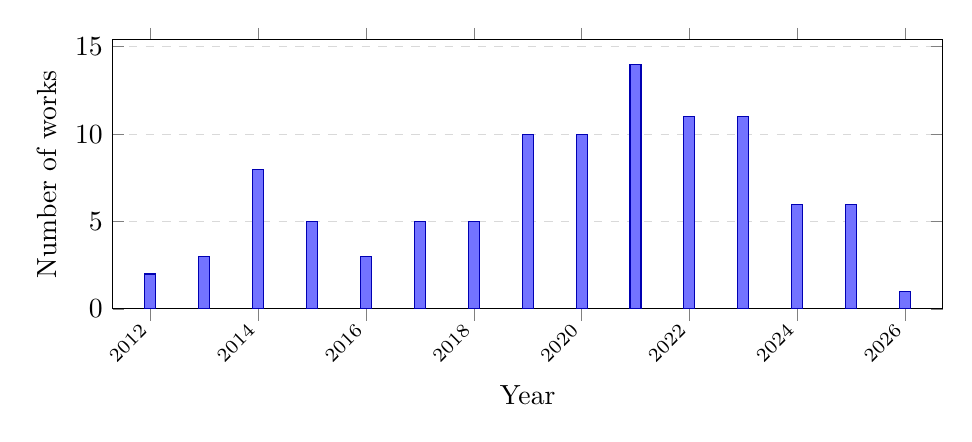
\begin{tikzpicture}
\begin{axis}[
  ybar, width=\columnwidth, height=5cm, bar width=4pt,
  xmin=2011.3, xmax=2026.7, ymin=0,
  xlabel={Year}, ylabel={Number of works},
  xtick distance=2, x tick label style={/pgf/number format/1000 sep=, rotate=45, anchor=east, font=\scriptsize},
  ymajorgrids, grid style={dashed,gray!30}, enlarge x limits=false]
\addplot[fill=blue!55, draw=blue!70!black] coordinates {(2012,2) (2013,3) (2014,8) (2015,5) (2016,3) (2017,5) (2018,5) (2019,10) (2020,10) (2021,14) (2022,11) (2023,11) (2024,6) (2025,6) (2026,1)};
\end{axis}
\end{tikzpicture}
\caption{Distribution of the surveyed works by publication year.}
\label{fig:years}
\end{figure}
\subsection{Cross-Cutting Trends in the Literature}
The temporal distribution of the surveyed corpus, shown in Fig.~\ref{fig:years}, reveals that interest in k-means clustering has been sustained over more than a decade, with the volume of work peaking in 2021 and a markedly steady stream of publications thereafter (13\% of the 100 works appeared in the last three years alone). This pattern suggests that k-means has not been superseded by newer paradigms but instead continues to be re-purposed and re-engineered: early work in the corpus concentrates on image segmentation pipelines \cite{dhanachandra2015image,wang2016method,shrivastava2014medical,suganya2013image}, while more recent contributions increasingly address algorithmic robustness \cite{khan2024addressing,xiao2024comprehensive}, principled model selection \cite{schubert2023stop,herdiana2026more,shi2021quantitative}, and scalability to big data settings \cite{mussabayev2025bimodalclust,mussabayev2023comparative}. The persistence of elbow-method papers across the whole timespan---from early heuristic applications \cite{syakur2018integration} to 2023--2026 attempts to formalize or critique the technique \cite{shi2021quantitative,herdiana2026more,schubert2023stop}---illustrates that even decades-old heuristics remain active sites of methodological contention rather than settled practice.

\subsection{Dominant Techniques and Convergent Themes}
Across the five thematic clusters identified in this survey, two technical concerns recur with striking consistency: initialization strategy and the choice of $k$. Initialization is treated as the primary lever for improving both convergence speed and clustering quality, whether through density- or kernel-based seeding \cite{kumar2017density,kumar2016color}, distance-based heuristics \cite{aldahdooh2013dimk,virmani2015normalization}, subtractive clustering \cite{dhanachandra2015image,tongbram2021segmentation}, or systematic comparisons of k-means++ against classical Forgy and random initialization \cite{li2018experiment,abdillah2025implementation,harris2022extensive,celebi2012comparative}. The empirical consensus from large-scale comparative studies \cite{franti2019how,harris2022extensive} is that careful initialization combined with repeated runs yields substantial accuracy gains over naive random seeding, a finding echoed in scalable variants such as global k-means++ \cite{vardakas2022global} and divide-and-conquer k-means++ \cite{hamalainen2020improving}. The second recurring concern, determining the number of clusters $k$, is dominated by the elbow method and its many hybridizations with k-means in domains ranging from customer segmentation \cite{syakur2018integration,tabianan2022means}, to healthcare \cite{wala2024heart}, education \cite{permadi2023means,ghifari2023clustering}, disaster management \cite{meliyana2025performance,ashari2023analysis}, and crime analytics \cite{sagala2022discovering}. Yet this dominance coexists with an emerging critical strand arguing that the elbow heuristic is statistically ill-posed and should be replaced by validity indices or more rigorous geometric criteria \cite{schubert2023stop,shi2021quantitative,herdiana2026more,ikotun2025cluster}, indicating a field in which popular practice and methodological rigor are not yet fully reconciled. A third convergent theme is the search for distance-metric and objective-function generalizations---including Canberra-based \cite{raeisi2022distance}, KROMD \cite{khan2024addressing}, weighted Euclidean \cite{zhao2021means}, and multi-view feature-weighted formulations \cite{yang2019feature,yang2023unsupervised}---that attempt to relax k-means' isotropic, spherical-cluster assumption, a limitation repeatedly flagged across surveys \cite{oti2021comprehensive,chong2021means,sattarov2023unveiling}.

\subsection{Datasets, Benchmarks, and Application Domains}
Unlike fields with standardized shared benchmarks, the k-means literature surveyed here is characterized by domain-specific, often bespoke datasets rather than common evaluation corpora. Image segmentation studies draw on medical imagery (MRI brain tumors \cite{alam2019automatic}, leukemia blood smears \cite{h2020leukemia,fatma2014leukemia}, prostate scans \cite{sammouda2021optimized}, cDNA microarrays \cite{wang2015improved}), remote sensing and environmental imagery (multi-spectral crop and marine satellite data \cite{kazakhstan2019multi,manahoran2017means}), and industrial or biological targets (metal abrasives \cite{zhang2023metal}, fruit \cite{wang2016method}, underwater scenes \cite{zhu2022means}), with comparatively few works reusing a shared public benchmark beyond occasional handwritten-digit datasets \cite{li2018experiment}. Similarly, the elbow-method and initialization literatures validate their proposals on heterogeneous tabular datasets---customer purchase records \cite{tabianan2022means,syakur2018integration}, sales data \cite{abdillah2025implementation}, school and disease records \cite{permadi2023means,wala2024heart}, and COVID-19 case statistics \cite{indraputra2020means}---chosen primarily for domain relevance rather than comparability across studies. The big-data and scalability cluster is the partial exception, where synthetic or large public datasets are used to stress-test throughput and memory behavior \cite{jain2014adapting,chen2019big,xie2020improvement,awad2022improved}, and where broader surveys of big-data platforms and infrastructure \cite{singh2014survey,tsai2015big,mahdi2021scalable} provide an implicit benchmarking context. This fragmentation of datasets across application domains limits direct cross-paper comparison and makes it difficult to assess whether reported algorithmic improvements generalize beyond the specific corpus or imaging modality on which they were demonstrated.

\subsection{Evaluation Practices}
Evaluation in the surveyed literature relies heavily on a small set of internal validity indices---silhouette score, Davies--Bouldin, Calinski--Harabasz, and variants of within-cluster sum of squares (the basis of the elbow method)---often used interchangeably or in combination without strong theoretical justification for the choice \cite{ashari2023analysis,sagala2022discovering,saputra2020effect,myagmarsuren2024exploring}. The comprehensive review of cluster validity indices \cite{ikotun2025cluster} and the critique of the elbow criterion \cite{schubert2023stop} both suggest that this reliance on a narrow, sometimes conflicting set of metrics is a weakness analogous to problems documented in other machine learning subfields, where surveys have shown that evaluation metrics can disagree substantially in their rankings of competing methods \cite{bi2024inconsistency,lee2023survey,srb2023navigating,terven2025comprehensive}. Few works in the k-means corpus report statistical significance testing or variance across multiple runs; instead, single-run silhouette or elbow plots are frequently treated as sufficient evidence of clustering quality \cite{myagmarsuren2024exploring,maori2023metode}. Where comparative rigor is pursued, it tends to appear in dedicated empirical studies, such as the systematic comparison of 17 initialization algorithms \cite{harris2022extensive}, the analysis of distance metrics' effect on k-value selection \cite{saputra2020effect,sthakare2015performance,ghazal2021performances}, and the large-scale investigation of initialization and repetition effects \cite{franti2019how}. This contrasts with the relative absence, in most application papers, of ablations isolating the contribution of a proposed modification (e.g., a new initialization or distance metric) from confounding factors such as dataset-specific preprocessing.

\subsection{Reproducibility and Open Challenges}
Reproducibility is a persistent concern across the corpus. Many application-oriented papers report only qualitative visual outcomes (e.g., segmented images) or single accuracy figures on proprietary or narrowly described datasets \cite{zhu2022means,zhang2023metal,wang2016method}, with limited detail on parameter settings, number of restarts, or convergence criteria, making independent replication difficult. Algorithmic-improvement papers are generally more transparent, often providing pseudocode or formal derivations for initialization \cite{aldahdooh2013dimk,kumar2017density,agha2012efficient} and optimization procedures \cite{zubair2022improved,zhao2022design}, yet code and data availability are inconsistently reported. The surveys and reviews in the corpus \cite{chong2021means,oti2021comprehensive,sattarov2023unveiling,mukherjee2025survey,mussabayev2023comparative} partially mitigate this by aggregating and re-contextualizing results, but they too note the difficulty of comparing heterogeneous experimental setups. Looking forward, the field would benefit from the kind of standardized benchmarking and metric taxonomies that have begun to emerge in adjacent machine learning areas \cite{terven2025comprehensive,srb2023navigating,benny2021evaluation}, alongside wider adoption of rigorous, multi-index model-selection practices \cite{ikotun2025cluster,schubert2023stop} and transparent reporting of initialization, runtime, and variance, so that the consid

\section{Open Challenges and Future Directions}\label{sec:challenges}
\subsection{Principled Selection of the Number of Clusters $K$}
A recurring obstacle across nearly every application of $k$-means is that the number of clusters must be fixed in advance, and the quality of the resulting partition is highly sensitive to this choice \cite{yuan2019research,chong2021means,gowsic2024enhanced,ran2021novel}. The elbow method, long used as a heuristic for selecting $K$, has recently been shown to lack theoretical justification, prompting calls to abandon it in favor of more principled alternatives \cite{schubert2023stop}. While numerous validity indices and quantitative elbow-detection schemes have been proposed to formalize this selection \cite{shi2021quantitative,herdiana2026more,ashari2023analysis,syakur2018integration,saputra2020effect}, and fully unsupervised variants attempt to discover $K$ automatically during optimization \cite{sinaga2020unsupervised,yang2023unsupervised,wei2013improved,hossain2019dynamic}, no consensus exists on which criterion is most reliable across data distributions, dimensionalities, and application domains. A promising direction is the development of theoretically grounded, data-adaptive stopping criteria that combine multiple validity signals and are empirically validated against ground truth across diverse benchmarks, rather than relying on a single heuristic curve.

\subsection{Sensitivity to Centroid Initialization}
Because $k$-means converges to a local optimum of a non-convex objective, its output is highly sensitive to the initial placement of centroids \cite{vardakas2022global,tongbram2021segmentation,xiao2024comprehensive,zubair2022improved}. Poor seeding can trap the algorithm in low-quality solutions, and this problem is compounded at scale, where repeated restarts become computationally prohibitive \cite{chen2019big}. Franti{\'\i}s and colleagues demonstrate that when clusters are well separated, final clustering quality is governed almost entirely by the goodness of initialization \cite{franti2019how}, underscoring that this is not a minor implementation detail but a central determinant of algorithm performance. Although a large body of work has proposed improved seeding strategies---density-based, distance-based, histogram-based, PCA-based, and relaxed global approaches \cite{kumar2017density,aldahdooh2013dimk,bhavani2022efficient,li2018experiment,agha2012efficient,vardakas2022global}---extensive empirical comparisons show no single method dominates across datasets and scenarios \cite{harris2022extensive}. Scalable divide-and-conquer initialization schemes \cite{hamalainen2020improving} and systematic initialization benchmarking \cite{celebi2012comparative} point toward a future in which initialization is treated as a first-class, dataset-adaptive design choice rather than a fixed default.

\subsection{Robustness to Outliers and Non-Spherical Cluster Structures}
The Euclidean, variance-minimizing formulation of $k$-means implicitly assumes convex, roughly spherical, and similarly sized clusters, which causes severe performance degradation when data contain outliers or non-globular structures \cite{shrifan2021adaptive,khan2024addressing}. Standard distance metrics also struggle to accommodate clusters of highly uneven density or shape \cite{raeisi2022distance}. Modified variants that incorporate outlier filtering, robust distance functions, or shape-aware transformations \cite{shrifan2021adaptive,khan2024addressing,shrivastava2014medical} show improvements, but typically address only one limitation at a time and often introduce new hyperparameters that themselves require tuning. This remains open because real-world data---medical images, sensor streams, behavioral records---rarely satisfy the spherical-cluster assumption, and there is no unified framework for jointly handling noise, shape irregularity, and density imbalance within the $k$-means paradigm. A fruitful direction is the integration of robust statistics and learned, data-driven distance metrics directly into the clustering objective, rather than as pre- or post-processing steps.

\subsection{Scalability to Big Data and Resource-Constrained Environments}
As dataset sizes and the desired number of clusters $K$ grow, $k$-means encounters a scalability bottleneck, since each iteration requires computing distances between all points and all centroids \cite{chen2019big,mahdi2021scalable}. This cost is further exacerbated in big-data applications where processing power and memory are limited \cite{awad2022improved}, and in image-based applications where computational cost grows with resolution \cite{lopez2014parallelization}. Although parallelization \cite{lopez2014parallelization}, bimodal optimization that fuses data- and neighborhood-level variation \cite{mussabayev2025bimodalclust}, distributed neural-processor implementations \cite{awad2022improved}, and energy-aware adaptations for constrained devices such as underwater sensor networks \cite{omeke2021dekcs} each mitigate specific bottlenecks, a general-purpose, provably scalable version of $k$-means that preserves clustering quality while operating under strict memory, energy, or latency budgets remains elusive. Continued progress will likely come from hybridizing approximate, sketch-based, or streaming computation with theoretically grounded quality guarantees, building on comparative surveys of existing optimization strategies \cite{mussabayev2023comparative}.

\subsection{Inconsistent and Task-Dependent Evaluation Practices}
Even when a clustering is produced, assessing its quality is far from settled. The silhouette score, one of the most widely used internal validity measures for $k$-means, has known limitations and does not always align with other $k$-means-specific metrics \cite{myagmarsuren2024exploring}, and broader empirical comparisons find it unclear which algorithm or evaluation criterion should be preferred in a given scenario \cite{harris2022extensive}. This difficulty is not unique to $k$-means: analogous evaluation-metric fragmentation has been documented in machine translation \cite{lee2023survey}, time-series anomaly detection \cite{srb2023navigating}, link prediction \cite{bi2024inconsistency}, topic modeling \cite{rudiger2022topic}, and deep learning broadly \cite{terven2025comprehensive}, suggesting a systemic gap in the field's ability to define task-appropriate, interpretable, and theoretically justified metrics. Comprehensive reviews of validity indices \cite{ikotun2025cluster} and multi-index comparison studies \cite{ashari2023analysis} represent initial steps, but a unified, context-sensitive evaluation methodology---potentially incorporating automated metric selection as proposed for other learning tasks \cite{terven2025comprehensive}---remains an open research direction for $k$-means specifically.

\subsection{Handling High-Dimensional, Multi-View, and Incomplete Data}
Standard $k$-means operates on a single, complete feature representation, yet modern data are frequently high-dimensional, multi-source, or partially missing. Most multi-view $k$-means algorithms cannot perform feature reduction during the clustering procedure itself, forcing an artificial separation between dimensionality reduction and cluster assignment \cite{yang2019feature}. Similarly, incomplete data traditionally require a separate imputation step before clustering can proceed, which can propagate imputation errors into the final partition \cite{wang2019means}. Unified objectives that jointly optimize feature weighting, imputation, and cluster assignment \cite{yang2019feature,wang2019means} show promise but remain comparatively underexplored relative to the vast literature on initialization and $K$-selection. Extending these joint formulations to automatically balance view importance, feature relevance, and missingness patterns---while retaining the computational simplicity that makes $k$-means attractive---constitutes an important avenue for future work.

\subsection{Theoretical Limits and Domain-Specific Adaptation}
Beyond practical heuristics, there exist fundamental theoretical

\section{Conclusion}\label{sec:conclusion}
\subsection{Conclusion}

This survey has organized the extensive literature on k-means clustering into six interrelated strands: applications to image segmentation, methods for determining the optimal number of clusters, centroid initialization and algorithmic refinements, broader surveys characterizing k-means variants, adaptations for big data, and the surrounding ecosystem of evaluation methodology and scalable analytics. Across these strands, a consistent picture emerges: the canonical k-means algorithm, despite its simplicity and enduring popularity, is rarely deployed in its original form. Practitioners and researchers routinely augment it with domain-specific initialization strategies (histogram-based, subtractive, or density-based), automated procedures for selecting $k$ (elbow-based heuristics, quantitative discriminant criteria, and unsupervised reformulations that bypass manual tuning altogether), and alternative distance metrics designed to handle uneven cluster sizes or improve robustness. The image segmentation literature illustrates this pattern vividly, where adaptive initialization and color-space transformations are used to overcome k-means' sensitivity to starting conditions and its implicit assumption of spherical, equally sized clusters. Similarly, the body of work on cluster-number selection shows a clear trajectory from the classical elbow heuristic toward more rigorous, automated, and geometrically grounded criteria, reflecting a broader push to reduce the subjectivity inherent in applying k-means.

A second major theme is scalability. As datasets have grown, a substantial body of research has focused on adapting k-means to big data settings through dimensionality reduction, approximate and fixed-iteration variants, distributed and hardware-accelerated implementations, and improved seeding algorithms such as scalable k-means++ and its relaxed global variants. These efforts collectively demonstrate that the computational bottlenecks of k-means---particularly the cost of good initialization and repeated distance computations---can be substantially mitigated without sacrificing clustering quality, though empirical comparisons show that no single optimization strategy dominates across all data regimes. Reviews of scalable clustering and big data analytics more broadly situate k-means within a larger ecosystem of methods, underscoring that its continued relevance stems from its favorable trade-off between interpretability, computational cost, and accuracy relative to more complex alternatives. The evaluation metrics literature, though largely developed outside the clustering context proper, reinforces a cautionary lesson applicable to k-means research: metric choice can materially affect conclusions about algorithmic performance, and inconsistency among metrics is a recurring risk that clustering validity studies must guard against.

Looking forward, several directions stand out as particularly important. First, there remains a need for principled, computationally cheap methods that jointly solve initialization and cluster-number selection rather than treating them as separate pipeline stages, since errors in one compound the other. Second, as learning-augmented approaches suggest, integrating predictive or learned signals into the clustering process offers a promising avenue for improving both speed and quality beyond purely heuristic initialization. Third, further work is needed on distance metrics and validity indices that generalize k-means beyond its native assumption of convex, isotropic clusters, extending the uneven-cluster and weighted-similarity efforts surveyed here. Finally, as big data and distributed/edge computing environments become the norm, scalable k-means variants must be evaluated not only for speed but for robustness and reproducibility under heterogeneous hardware and streaming conditions, an area where current empirical comparisons remain fragmented. Addressing these directions will be essential to sustaining k-means as a

\bibliographystyle{IEEEtran}
\bibliography{refs}
\end{document}
